\documentclass{cekarticle}
\usepackage{color}
\usepackage{amsmath}
\usepackage{amssymb}
\usepackage{array}

\begin{document}

%=============================================================================
% Title page
%=============================================================================

\title{Systems Biology Markup Language (SBML) Level 3 Proposal: Multi-component Species Features}

\author{Andrew Finney}

\authoremail{
\begin{minipage}{\textwidth}\centering
afinney@cds.caltech.edu
\end{minipage}}

\maketitlepage

%\section{Executive Summary}
%\label{Executive Summary}

%=============================================================================
\section{Terms of Reference}
\label{sec:t-o-r}
%=============================================================================

This document describes proposed features for inclusion in Systems
Biology Markup Language (SBML) Level 3. This document describes
features enabling the description of large chemical entities that
are composed from other chemical entities.  (Entities of this type
were previously classed as `complex species'. This term is
confusing~\citep{phair:2003} and is avoided in this document.)

This document is not a definition of SBML Level 3 or part of it.
This document simply presents various features which could be
incorporated into SBML Level 3 as the Systems Biology community
wishes.  This document is intended for detailed review by that
community and to provoke alternative proposals.

This document is not the first proposal to support multi-component species~\citep{lenovere:2002}
and supersedes a previous proposal by the author~\citep{finney:2001f}.

Throughout this
document issues that the author believes will require further
discussion have been highlighted.

For brevity the text of this document is with reference to SBML
Level 2~\citep{finney:2002f} i.e. features are described in terms
of changes to SBML Level 2.  In addition for brevity the UML diagrams in this proposal
show only new attributes and types for SBML Level 3.

All types proposed in this document will be derived from the
\texttt{SBase} type.


\section{Acknowledgements}

This proposal has benefitted from discussions the author had with
Martin Ginkel, J\"org Stelling, Nicolas Le Novere, Fabian
Campagne, Jeremy Zucker, Robert Phair, Larry Lok, Michael Blinov
and Roger Brent. In particular many of the ideas presented here
are similar to those developed by the Molecular Sciences Institute
and the T-10 Cell Signalling Group~\citep{goldstein:2001} at Los
Alamos National Laboratories.

Support for the development of this proposal came from the
following the National Human Genome Research Institute (USA) and
the Japan Science and Technology Corporation under the ERATO
Kitano Symbiotic Systems Project. Additional support was provided
by the California Institute of Technology (USA), the University of
Hertfordshire (UK) and the Molecular Sciences Institute (USA).

\section{Aims}

This proposal aims to support the representation of the following concepts that are not easily
represented in SBML Level 2:

\begin{itemize}
\item the common description of biochemical entities that can then be located in different
compartments
\item the common description of biochemical reactions that can then be located in different
compartments
\item the hierarchical description of biochemical entities through the composition of other
biochemical entities
\item the description of biochemical entities through simple associative composition
\item the description of biochemical entities through graphs of other biochemical entities
where arcs represent kinds of bonding
\item the description of generalized biochemical reactions that avoids the enumeration of
many species states and reactions
\end{itemize}

In particular this proposal aims to enable the description of, for example, proteins which
can contain many phosphorylation states,
complexes of these proteins and models of signalling pathways which contain these proteins.

\clearpage

\section{Overview of Proposal}

A UML diagram for the proposed new classes is shown in
figures~\ref{fig:multi-component-species-uml}
and~\ref{fig:multi-component-species-uml2}.
Section~\ref{sec:tutorial} demonstrates with examples, how
instances of these classes can be assembled to achieve the aims of
the proposal.  Section~\ref{sec:tutorial} effectively defines a
staged road map of how the features described in this proposal
could be added to SBML. The proposal is described more formally in
section~\ref{sec:definitions}. Section~\ref{sec:definitions} can
be considered as a reference section.
%The Appendix includes tables which summarize the new XML components that
%are introduced by this proposal to the XML encoding of SBML.


\begin{figure}[h]
  \vspace*{8pt}
  \centering
  \includegraphics[scale = 0.7]{multi-component-species-uml.eps}
  \caption{The types and attributes introduced into SBML by this proposal.  This diagram
  only shows new classes and fields: all SBML Level 2 structures are assumed to be present.
  This diagram is continued in Figure~\ref{fig:multi-component-species-uml2}}
  \label{fig:multi-component-species-uml}
\end{figure}
\begin{figure}[h]
  \vspace*{8pt}
  \centering
  \includegraphics[scale = 0.7]{multi-component-species-uml2.eps}
  \caption{The types and attributes introduced into SBML by this proposal.  This diagram
  only shows new classes and fields: all SBML Level 2 structures are assumed to be present.
  This diagram is a continuation of the diagram in Figure~\ref{fig:multi-component-species-uml}}
  \label{fig:multi-component-species-uml2}
\end{figure}

\clearpage

\section{Tutorial on the Proposed Features}
\label{sec:tutorial}

\subsection{Terminology}

The following terminology is used in this document:
\begin{itemize}
\item \emph{chemical entity} any individual chemical object
  e.g. a calcium ion, a phosphate, a protein, and a lipid.

\item \emph{compartment} a well stirred container of chemical entities

\item \emph{species type} a type of chemical entity,
  specifically a set of chemical entities with exactly the same chemical form,

\item \emph{species} a pool of chemical entities of the same species type located in a
  specific compartment
\end{itemize}

\subsection{The Definition of Chemical Entities across Compartments}
\label{sec:commonspecies}

Consider a model where we have a species type which exists in more than one compartment.
For example we might wish to model Aspartate in a Cytosol compartment and in the Mitochondrial Matrix.
In SBML Level 2 we have to explicitly define each pool of Aspartate located in a separate compartment,
using a \class{Species} structure as shown in Figure~\ref{fig:malate_aspartate_shuttle1-xml}

\begin{figure}[h]
\begin{example}
<model id="malate_aspartate_shuttle1">
    <listOfCompartments>
        <compartment id="Cytosol"/>
        <compartment id="Mitochondrial_Matrix"/>
    </listOfCompartments>
    <listOfSpecies>
        <species id="Aspartate_in_Cytosol" compartment="Cytosol"/>
        <species id="Aspartate_in_Mitochondrial_Matrix" compartment="Mitochondrial_Matrix"/>
    </listOfSpecies>
</model>
\end{example}
\caption{\texttt{malate\_aspartate\_shuttle1} Model with the same type of chemical entity located in
different compartments.}
\label{fig:malate_aspartate_shuttle1-xml}
\end{figure}

In SBML Level 2 there is no formal way to relate these species together.  Under this proposal
we can do this by representing a chemical entity type such as, Aspartate,
with a \class{SpeciesType} structure and then
refer to the \class{SpeciesType} from the \class{Species} structures.  We can thus transform the
\texttt{malate\_aspartate\_shuttle1} Model in Figure~\ref{fig:malate_aspartate_shuttle1-xml} to that
shown in Figure~\ref{fig:malate_aspartate_shuttle2-xml}.

\begin{figure}[h]
\begin{example}
<model id="malate_aspartate_shuttle2">
    <listOfCompartments>
        <compartment id="Cytosol"/>
        <compartment id="Mitochondrial_Matrix"/>
    </listOfCompartments>
    <listOfSpeciesTypes>
        <speciesType id="Aspartate"/>
    </listOfSpeciesTypes>
    <listOfSpecies>
        <species
            id="Aspartate_in_Cytosol"
            speciesType="Aspartate"
            compartment="Cytosol"/>
        <species
            id="Aspartate_in_Mitochondrial_Matrix"
            speciesType="Aspartate"
            compartment="Mitochondrial_Matrix"/>
    </listOfSpecies>
</model>
\end{example}
\caption{\texttt{malate\_aspartate\_shuttle2} Model which uses a \class{SpeciesType} to link species of
the same type of chemical entity that are located in different compartments.}
\label{fig:malate_aspartate_shuttle2-xml}
\end{figure}

This model does not introduce any new variables that are not present in
\texttt{malate\_aspartate\_shuttle1} it simply identifies \texttt{Aspartate\_in\_Cytosol}
and \texttt{Aspartate\_in\_Mitochondrial\_Matrix} as being separate pools of the same chemical entity.
You cannot refer to \class{SpeciesType} structures from MathML structures under this proposal.

The \texttt{malate\_aspartate\_shuttle1} example is still a valid model under this proposal.
For backwards compatibility the \attrib{speciesType} attribute on \class{Species} is not
mandatory.

It is not possible to locate a \class{SpeciesType} in a
\class{Compartment} more than once, for example, it is not
possible for two \class{Species} structures to have the same
\attrib{speciesType} and \attrib{compartment} values.

\subsection{Generalized Reactions: The Definition of Reactions across Compartments}
\label{sec:commonreaction}

Just as we might wish to give a common identify to chemical entities distributed across several
compartments we might wish to have some common object describing reactions between those chemical
entities that is independent of the compartments in which the reactions occur.

For example consider the representation of the transamination reaction, a reversible reaction
that converts Aspartate to Oxaloacetate in both the Cytosol and Mitochondrial Matrix.

We could extend \texttt{malate\_aspartate\_shuttle2} using
\class{SpeciesType} structures combined with other SBML Level 2
structures the SBML Level 2 form as shown in
Figure~\ref{fig:malate_aspartate_shuttle3-xml} on
page~\pageref{fig:malate_aspartate_shuttle3-xml}. Under this
proposal we can replace the 2 reactions in
Figure~\ref{fig:malate_aspartate_shuttle3-xml} with a single
reaction structure as shown in
Figure~\ref{fig:malate_aspartate_shuttle4-xml} on
page~\pageref{fig:malate_aspartate_shuttle4-xml}.

\begin{figure}[h]
\begin{example}
<model id="malate_aspartate_shuttle3">
    <listOfCompartments>
        <compartment id="Cytosol"/>
        <compartment id="Mitochondrial_Matrix"/>
    </listOfCompartments>
    <listOfSpeciesTypes>
        <speciesType id="Aspartate"/>
        <speciesType id="Oxaloacetate"/>
    </listOfSpeciesTypes>
    <listOfSpecies>
        <species
            id="Aspartate_in_Cytosol"
            speciesType="Aspartate"
            compartment="Cytosol"/>
        <species
            id="Aspartate_in_Mitochondrial_Matrix"
            speciesType="Aspartate"
            compartment="Mitochondrial_Matrix"/>
        <species
            id="Oxaloacetate_in_Cytosol"
            speciesType="Oxaloacetate"
            compartment="Cytosol"/>
        <species
            id="Oxaloacetate_in_Mitochondrial_Matrix"
            speciesType="Oxaloacetate"
            compartment="Mitochondrial_Matrix"/>
    </listOfSpecies>
    <listOfReactions>
        <reaction id="Transamination_in_Cytosol" reversible="true">
            <listOfReactants>
                <speciesReference species="Aspartate_in_Cytosol"/>
            </listOfReactants>
            <listOfProducts>
                <speciesReference species="Oxaloacetate_in_Cytosol"/>
            </listOfProducts>
        </reaction>
        <reaction id="Transamination_in_Mitochondrial_Matrix" reversible="true">
            <listOfReactants>
                <speciesReference species="Aspartate_in_Mitochondrial_Matrix"/>
            </listOfReactants>
            <listOfProducts>
                <speciesReference species="Oxaloacetate_in_Mitochondrial_Matrix"/>
            </listOfProducts>
        </reaction>
    </listOfReactions>
</model>
\end{example}
\caption{The \texttt{malate\_aspartate\_shuttle3} model which has duplicate reactions for each
compartment.}
\label{fig:malate_aspartate_shuttle3-xml}
\end{figure}

\begin{figure}[h]
\begin{example}
<model id="malate_aspartate_shuttle4">
    <listOfCompartments>
        <compartment id="Cytosol"/>
        <compartment id="Mitochondrial_Matrix"/>
    </listOfCompartments>
    <listOfSpeciesTypes>
        <speciesType id="Aspartate"/>
        <speciesType id="Oxaloacetate"/>
    </listOfSpeciesTypes>
    <listOfSpecies>
        <species
            id="Aspartate_in_Cytosol"
            speciesType="Aspartate"
            compartment="Cytosol"/>
        <species
            id="Aspartate_in_Mitochondrial_Matrix"
            speciesType="Aspartate"
            compartment="Mitochondrial_Matrix"/>
        <species
            id="Oxaloacetate_in_Cytosol"
            speciesType="Oxaloacetate"
            compartment="Cytosol"/>
        <species
            id="Oxaloacetate_in_Mitochondrial_Matrix"
            speciesType="Oxaloacetate"
            compartment="Mitochondrial_Matrix"/>
    </listOfSpecies>
    <listOfReactions>
        <reaction id="Transamination" reversible="true">
            <listOfReactants>
                <speciesReference speciesType="Aspartate"/>
            </listOfReactants>
            <listOfProducts>
                <speciesReference speciesType="Oxaloacetate"/>
            </listOfProducts>
        </reaction>
    </listOfReactions>
</model>
\end{example}
\caption{The \texttt{malate\_aspartate\_shuttle4} model which has a single reaction which is potentially
located in all compartments.}
\label{fig:malate_aspartate_shuttle4-xml}
\end{figure}

All the \class{SimpleSpeciesReference} structures (that is
modifiers, reactants and products) refer to species in the same
compartment.  This means that, under this proposal, it is not
possible to define a transport reaction, that is a reaction which
moves chemical entities between compartments, using this form.

\subsubsection{Defining the explicit location of a \class{SimpleSpeciesReference}}
\label{sec:locatedspeciesreferences}

The location of a species pool can be made explicit in a
\class{SimpleSpeciesReference} structure without referring to a
\class{Species} structure.  This can be achieved by using the
proposed optional \attrib{compartment} field which refers to a
\class{Compartment} structure to indicate the location of the
given \class{SpeciesType}. For example consider the transport
reaction shown in Figure~\ref{fig:Malate_Transport-xml} on
page~\pageref{fig:Malate_Transport-xml} which can be added to the
model in Figure~\ref{fig:malate_aspartate_shuttle4-xml} on
page~\pageref{fig:malate_aspartate_shuttle4-xml}.

\begin{figure}[h]
\begin{example}
<reaction id="Malate_Transport" reversible="false">
    <listOfReactants>
        <speciesReference speciesType="Malate" compartment="Cytosol"/>
    </listOfReactants>
    <listOfProducts>
        <speciesReference speciesType="Malate" compartment="Mitochondrial_Matrix"/>
    </listOfProducts>
</reaction>
\end{example}
\caption{The \texttt{Malate\_Transport} model a transport reaction which refers to \class{SpeciesType}
structures in specific compartments.}
\label{fig:Malate_Transport-xml}
\end{figure}

All the \class{SimpleSpeciesReference} structures of a reaction
should simultaneously either (a) be located (i.e. have values for
the \attrib{species} or \attrib{compartment} attributes); or (b)
apply to any compartment (i.e. not have values for the
\attrib{species} and \attrib{compartment} attributes). \emph{This
restriction is not essential but simplifies the interpretation of
the proposed format}.

\emph{This feature could be introduced later in the SBML
development road map. It is however an essential component of
features introduced later.}

\subsubsection{Defining Kinetic Laws for Generalized Reactions}

As defined in the examples above it is not possible to compose the kinetic law of these generalized
reactions since there is no symbol that refers to either the modifiers, reactants or products or the
reaction species pools.  However under this proposal the \attrib{id} field of a
\class{SimpleSpeciesReference} becomes a symbol that can be used in the \class{KineticLaw} of the
enclosing \class{Reaction}.

\emph{Here I am assuming that the \attrib{id} field on \class{SimpleSpeciesReference} is introduced by a
new version of SBML Level 2. This \attrib{id} field is in the global symbol
namespace despite, for the purposes of this proposal, only having scope in the enclosing
\class{Reaction}.  If this is problematic then perhaps we could consider an additional attribute to
declare the symbol.}

As example Figure~\ref{fig:Transamination-xml} on
page~\pageref{fig:Transamination-xml} shows the
\texttt{Transamination} reaction, from model
\texttt{malate\_aspartate\_shuttle4}, modified to include a rate
law.

\begin{figure}[h]
\begin{example}
<reaction id="Transamination" reversible="true">
    <listOfReactants>
        <speciesReference id="S1" speciesType="Aspartate"/>
    </listOfReactants>
    <listOfProducts>
        <speciesReference speciesType="Oxaloacetate"/>
    </listOfProducts>
    <kineticLaw>
        <math xmlns="http://www.w3.org/1998/MathMathML">
            <apply>
                <times/>
                <cn>1.1</cn>
                <ci>S1</ci>
            </apply>
        </math>
    </kineticLaw>
</reaction>
\end{example}
\caption{The \texttt{Transamination} reaction from
Figure~\ref{fig:malate_aspartate_shuttle4-xml} modified to include a kinetic law.}
\label{fig:Transamination-xml}
\end{figure}

\subsubsection{The Unit Attributes of \class{SimpleSpeciesReference}}

To make the units of species explicit in kinetic laws under this
proposal \class{SimpleSpeciesReference} structures have the
attributes \attrib{substanceUnits}, \attrib{spatialSizeUnits} and
\attrib{hasOnlySubstanceUnits}.  These have the same semantics as
the corresponding attributes on \class{Species}.

\subsection{Species Implied from \class{SpeciesTypes}}

Under this proposal \class{Species} structures are used to
indicate the initial conditions and/or attributes of species and
don't represent the complete set of species.  In fact this
proposal does not assume that an interpreter (e.g. simulator) of
models in the proposed format would use species as it's
fundamental representational form, for example an interpreter may
represent individual chemical entities as distinct objects. In
SBML Level 2 the model's \attrib{species} list is a complete
enumeration of the pools of chemical entities.  In this proposal
this set of species is a subset of the complete set of species
defined by the model. The remaining species are implied by
\class{SpeciesType} structures, as described in this section, or
are implied by reactions generalized to cover classes of
\class{SpeciesTypes}, see Section~\ref{sec:generalizedreactions}.

For each \class{SpeciesType} there exists a species of the given
type in each compartment in the model unless there already exists
an equivalent \class{Species} structure located in that
compartment.  These implied species always have an initial
concentration or substance amount of zero and are never constant
nor boundary conditions. This means that constant or boundary
condition species or species with any initial concentration must
be made explicit using a \class{Species} structure.

So if we consider the model \texttt{malate\_aspartate\_shuttle4}
on page~\pageref{fig:malate_aspartate_shuttle4-xml} we can omit
any species structures which we wish to model as having an initial
concentration of zero.   This is shown in
Figure~\ref{fig:malate_aspartate_shuttle5-xml} where we assume
that only \class{Aspartate} species have an initial concentration.

\begin{figure}[h]
\begin{example}
<model id="malate_aspartate_shuttle5">
    <listOfCompartments>
        <compartment id="Cytosol"/>
        <compartment id="Mitochondrial_Matrix"/>
    </listOfCompartments>
    <listOfSpeciesTypes>
        <speciesType id="Aspartate"/>
        <speciesType id="Oxaloacetate"/>
    </listOfSpeciesTypes>
    <listOfSpecies>
        <species
            id="Aspartate_in_Cytosol"
            speciesType="Aspartate"
            compartment="Cytosol"
            initialConcentration="1"/>
        <species
            id="Aspartate_in_Mitochondrial_Matrix"
            speciesType="Aspartate"
            compartment="Mitochondrial_Matrix"
            initialConcentration="1"/>
    </listOfSpecies>
    <listOfReactions>
        <reaction id="Transamination" reversible="true">
            <listOfReactants>
                <speciesReference speciesType="Aspartate"/>
            </listOfReactants>
            <listOfProducts>
                <speciesReference speciesType="Oxaloacetate"/>
            </listOfProducts>
        </reaction>
    </listOfReactions>
</model>
\end{example}
\caption{The \texttt{malate\_aspartate\_shuttle5} model with a
reduced set of \texttt{Species} structures.}
\label{fig:malate_aspartate_shuttle5-xml}
\end{figure}


\emph{The concept of implied species could be introduced later in the SBML development road map.
It is however an essential component of features introduced later.}

\subsection{Simple Multi-Component Chemical Entities}
\label{sec:multicomponentspecies}

In this proposal \class{SpeciesType} structures can be composed
from instances of other \class{SpeciesType} structures. These
instances are encoded as \class{SpeciesTypeInstance} structures.
For example see the \texttt{Pheromone\_Response} model, shown with
XML and diagram form in Figure~\ref{fig:pheromone_response}.

\begin{figure}[h]
\begin{example}
<model "Pheromone_response">
    <listOfSpeciesTypes>
        <speciesType id="Ste5"/>
        <speciesType id="Ste11"/>
        <speciesType id="Ste7"/>
        <speciesType id="Fus3"/>
        <speciesType id="SteComplex">
            <listOfSpeciesTypeInstances>
                <speciesTypeInstance id="iSte5" speciesType="Ste5"/>
                <speciesTypeInstance id="iSte11" speciesType="Ste11"/>
                <speciesTypeInstance id="iSte7" speciesType="Ste7"/>
                <speciesTypeInstance id="iFus3" speciesType="Fus3"/>
            </listOfSpeciesTypeInstances>
        </speciesType>
    </listOfSpeciesTypes>
</model>
\end{example}
  \vspace*{8pt}
  \centering
  \includegraphics[scale = 0.7]{pheromone_response.eps}
  \caption{The \texttt{Pheromone\_response} model}
  \label{fig:pheromone_response}
\end{figure}

This indicates that \texttt{SteComplex} is a complex made up of
one instance each of the proteins \texttt{Ste5}, \texttt{Ste11},
\texttt{Ste7} and \texttt{Fus3}.  The individual instances are
always identified to enable the components of homodimers to be
separately identified.  In the diagram a rectangle not enclosed
within another rectangle represents a \class{SpeciesType}
structure. A rectangle with a normal typeface label represents a
\class{SpeciesTypeInstance} structure and is enclosed within a box
representing a \class{SpeciesType}.

We can also describe reactions in using this form on
\class{SpeciesReference} structures.  For example we can describe
the binding of \texttt{Ste11} to \texttt{Ste5} with the
\class{Reaction} structure shown in
Figure~\ref{fig:binding_Ste5_Ste11}. In this diagram the rectangle
without italic along the top edge represent a
\class{SimpleSpeciesReference} structure which contains one or
more \class{SpeciesTypeInstance} structures.

\begin{figure}[h]
\begin{example}
<reaction id="binding_Ste5_Ste11">
    <listOfReactants>
        <speciesReference speciesType="Ste11"/>
        <speciesReference speciesType="Ste5"/>
    </listOfReactants>
    <listOfProducts>
        <speciesReference>
            <listOfSpeciesTypeInstances>
                <speciesTypeInstance id="iSte5" speciesType="Ste5"/>
                <speciesTypeInstance id="iSte11" speciesType="Ste11"/>
            </listOfSpeciesTypeInstances>
        </speciesReference>
    </listOfProducts>
</reaction>
\end{example}
  \vspace*{8pt}
  \centering
  \includegraphics[scale = 0.7]{binding_Ste5_Ste11.eps}
  \caption{The \texttt{binding\_Ste5\_Ste11} reaction, operating in the context of the species types
  defined in Figure~\ref{fig:pheromone_response}.  This indicates that the reaction
  \texttt{binding\_Ste5\_Ste11} creates a complex consisting of \texttt{Ste5} and \texttt{Ste11} entities
  form unbound \texttt{Ste5} and \texttt{Ste11} entities.}
  \label{fig:binding_Ste5_Ste11}
\end{figure}

Although the identity of \class{SpeciesTypeInstance} structures is
declared in each \class{SimpleSpeciesReference} structure these
identities have scope throughout a reaction. The
\class{SpeciesTypeInstance} \attrib{id} fields with the same value
in the same reaction refer to the same chemical entity.  By giving
\class{SpeciesTypeInstance} \attrib{id} fields the same values in
the reactants and products of a reaction we indicate that the
entity is only modified by the reaction rather than being created
or destroyed by the reaction.  For example the reaction
\texttt{binding\_Ste5\_Ste11} could be encoded as shown in
Figure~\ref{fig:binding_Ste5_Ste11_v2}.

\begin{figure}[h]
\begin{example}
<reaction id="binding_Ste5_Ste11_v2">
    <listOfReactants>
        <speciesReference>
            <listOfSpeciesTypeInstances>
                <speciesTypeInstance id="iSte5" speciesType="Ste5"/>
            </listOfSpeciesTypeInstances>
        </speciesReference>
        <speciesReference>
            <listOfSpeciesTypeInstances>
                <speciesTypeInstance id="iSte11" speciesType="Ste11"/>
            </listOfSpeciesTypeInstances>
        </speciesReference>
    </listOfReactants>
    <listOfProducts>
        <speciesReference>
            <listOfSpeciesTypeInstances>
                <speciesTypeInstance id="iSte5" speciesType="Ste5"/>
                <speciesTypeInstance id="iSte11" speciesType="Ste11"/>
            </listOfSpeciesTypeInstances>
        </speciesReference>
    </listOfProducts>
</reaction>
\end{example}
  \vspace*{8pt}
  \centering
  \includegraphics[scale = 0.7]{binding_Ste5_Ste11_v2.eps}
  \caption{The \texttt{binding\_Ste5\_Ste11\_v2} reaction}
  \label{fig:binding_Ste5_Ste11_v2}
\end{figure}

This encoding indicates that, for the purposes of the model,
\texttt{Ste5} and \texttt{Ste11} are not modified when they bond.
The distinction between \texttt{binding\_Ste5\_Ste11} and
\texttt{binding\_Ste5\_Ste11\_v2} is only descriptive however the
latter form is used as the basis for more complex semantics later.
A model like \texttt{pheromone\_response} with or without
characterized reactions including kinetic laws doesn't encapsulate
a model that can be simulated because it does not specify any
species of non-zero concentration.

\subsection{Multi-component Chemical Entities with explicit bonds}
\label{sec:explicitbonds}

The forms described in section~\ref{sec:multicomponentspecies}
capture some but not all the relevant knowledge of chemical
entities that we might wish to model.  In this section I describe
how chemical bond information is captured. The bond information on
a \class{SimpleSpeciesReference} or a \class{SpeciesType} is a
graph linking the \class{SpeciesTypeInstance} structures together.
The description of a structure using chemical bonds requires the
identification of binding sites on \class{SpeciesType} structures,
using \class{BindingSite} structures, and then the enumeration of
the bonds on those binding sites using \class{SpecificBond}
structures. \class{SpecificBond} structures consist of pairs of
\class{BindingSiteReference} structures. We can redefine the model
\texttt{pheromone\_response} along these lines as shown in
Figure~\ref{fig:pheromone_response_v2} on
page~\pageref{fig:pheromone_response_v2}.  In the diagram the
lines perpendicular to the outer edge of \class{SpeciesType}
structures represent \class{BindingSite} structures.
\class{SpecifcBond} structures are represented as lines joining
\class{SpeciesTypeInstance} structures.

\begin{figure}[h]
\begin{example}
<model "pheromone_response_v2">
    <listOfSpeciesTypes>
        <speciesType id="Ste5">
            <listOfBindingSites>
                <bindingSite id="r241">
                <bindingSite id="r463">
                <bindingSite id="r744">
            </listOfBindingSites>
        </speciesType>
        <speciesType id="Ste11"/>
            <listOfBindingSites>
                <bindingSite id="site">
            </listOfBindingSites>
        </speciesType>
        <speciesType id="Ste7"/>
            <listOfBindingSites>
                <bindingSite id="site">
            </listOfBindingSites>
        </speciesType>
        <speciesType id="Fus3"/>
            <listOfBindingSites>
                <bindingSite id="site">
            </listOfBindingSites>
        </speciesType>
        <speciesType id="SteComplex">
            <listOfSpeciesTypeInstances>
                <speciesTypeInstance id="iSte5" speciesType="Ste5"/>
                <speciesTypeInstance id="iSte11" speciesType="Ste11"/>
                <speciesTypeInstance id="iSte7" speciesType="Ste7"/>
                <speciesTypeInstance id="iFus3" speciesType="Fus3"/>
            </listOfSpeciesTypeInstances>
            <listOfBonds>
                <specificBond>
                    <bindingSiteReference speciesTypeInstance="iSte5" bindingSite="r241"/>
                    <otherBindingSiteReference
                        speciesTypeInstance="iFus3" bindingSite="site"/>
                </specificBond>
                <specificBond>
                    <bindingSiteReference speciesTypeInstance="iSte5" bindingSite="r463"/>
                    <otherBindingSiteReference
                        speciesTypeInstance="iSte11" bindingSite="site"/>
                </specificBond>
                <specificBond>
                    <bindingSiteReference speciesTypeInstance="iSte5" bindingSite="r744"/>
                    <otherBindingSiteReference
                        speciesTypeInstance="iSte7" bindingSite="site"/>
                </specificBond>
            </listOfBonds>
        </speciesType>
    </listOfSpeciesTypes>
</model>
\end{example}
  \vspace*{8pt}
  \centering
  \includegraphics[scale = 0.7]{pheromone_response_v2.eps}
  \caption{The
  \texttt{pheromone\_response\_v2}
  model which demonstrates the use of \class{BindingSite} and \class{SpecificBond} structures.}
  \label{fig:pheromone_response_v2}
\end{figure}

\class{SpecificBond} structures can be used to indicate unbound
binding sites, simply by containing a single
\class{BindingSiteReference} structure, as shown the reaction in
Figure~\ref{fig:binding_Ste5_Ste11_v3} on
page~\pageref{fig:binding_Ste5_Ste11_v3}.  In this diagram unbound
binding sites are represented as disconnected lines perpendicular
to the edge of a \class{SpeciesTypeInstance}.  A
\class{SpeciesType} structure must not leave the state of a
binding site undefined or ambiguous.
Section~\ref{sec:generalizedreactions} describes how a
\class{SimpleSpeciesReference} can refer to several different
\class{SpeciesType} structures where the class represents a range
of states for one or more binding sites.

\begin{figure}[h]
\begin{example}
<reaction id="binding_Ste5_Ste11_v3">
    <listOfReactants>
        <speciesReference>
            <listOfSpeciesTypeInstances>
                <speciesTypeInstance id="iSte5" speciesType="Ste5"/>
            </listOfSpeciesTypeInstances>
            <listOfBonds>
                <specificBond>
                    <bindingSiteReference speciesTypeInstance="iSte5" bindingSite="r241"/>
                </specificBond>
                <specificBond>
                    <bindingSiteReference speciesTypeInstance="iSte5" bindingSite="r463"/>
                </specificBond>
                <specificBond>
                    <bindingSiteReference speciesTypeInstance="iSte5" bindingSite="r744"/>
                </specificBond>
            </listOfBonds>
        </speciesReference>
        <speciesReference>
            <listOfSpeciesTypeInstances>
                <speciesTypeInstance id="iSte11" speciesType="Ste11"/>
            </listOfSpeciesTypeInstances>
            <listOfBonds>
                <specificBond>
                    <bindingSiteReference speciesTypeInstance="iSte11" bindingSite="site"/>
                </specificBond>
            </listOfBonds>
         </speciesReference>
    </listOfReactants>
    <listOfProducts>
        <speciesReference>
            <listOfSpeciesTypeInstances>
                <speciesTypeInstance id="iSte5" speciesType="Ste5"/>
                <speciesTypeInstance id="iSte11" speciesType="Ste11"/>
            </listOfSpeciesTypeInstances>
            <listOfBonds>
                <specificBond>
                    <bindingSiteReference speciesTypeInstance="iSte5" bindingSite="r241"/>
                </specificBond>
                <specificBond>
                    <bindingSiteReference speciesTypeInstance="iSte5" bindingSite="r463"/>
                    <otherBindingSiteReference
                        speciesTypeInstance="iSte11" bindingSite="site"/>
                </specificBond>
                <specificBond>
                    <bindingSiteReference speciesTypeInstance="iSte5" bindingSite="r744"/>
                </specificBond>
            </listOfBonds>
        </speciesReference>
    </listOfProducts>
</reaction>
\end{example}
  \vspace*{8pt}
  \centering
  \includegraphics[scale = 0.7]{binding_Ste5_Ste11_v3.eps}
  \caption{The \texttt{binding\_Ste5\_Ste11\_v3} reaction which demonstrates the
  representation of unbound states. For example \class{BindingSite} \texttt{r744} on
  \class{SpeciesTypeInstance} \texttt{iSte5} is unbound before and after the reaction}
  \label{fig:binding_Ste5_Ste11_v3}
\end{figure}

The level of decomposition of a biochemical system into chemical entities and their binding sites and
bonds is not defined by this proposal.  This proposal is designed to support arbitrary decomposition
schemes which capture knowledge at different resolutions in the same model. The
underlying chemistry represented by a given binding site state is also not defined by this proposal.

An underlying principle of this proposal is that the binding
representation described in this section can be used to represent
the reversible covalent modification of proteins including, for
example, phosphorylation and dephosphorylation.  The example model
shown in Figure~\ref{fig:Phosphorylation_model-xml} on
page~\pageref{fig:Phosphorylation_model-xml} represents the
phosphorylation of \texttt{Ste11} by \texttt{Ste20}.  A diagram of
this model is shown in Figure~\ref{fig:Phosphorylation_model} on
page~\pageref{fig:Phosphorylation_model}.  This digram is divided
into two parts by a horizontal lines.  The objects above the line
represent the \class{SpeciesTypes} in the model and the rest of
the diagram represents the reaction in the model.  The object
parallel to the reaction arrow represents the reaction's modifier.

\begin{figure}[h]
\begin{example}
<model id="Phosphorylation_model">
    <listOfSpeciesTypes>
        <speciesType id="Phosphate">
            <listOfBindingSites>
                <bindingSite id="site"/>
            </listOfBindingSites>
        </speciesType>
        <speciesType id="Ste20"/>
        <speciesType id="Ste11">
            <listOfBindingSites>
                <bindingSite id="S302"/>
                <bindingSite id="T307"/>
            </listOfBindingSites>
        </speciesType>
    </listofSpeciesTypes>
    <listOfReactions>
        <reaction id="Phosphorylation">
            <listOfReactants>
                <speciesReference>
                    <listOfSpeciesTypeInstances>
                        <speciesTypeInstance id="iSte11" speciesType="Ste11"/>
                    </listOfSpeciesTypeInstances>
                    <listOfBonds>
                        <specificBond>
                            <bindingSiteReference
                                speciesTypeInstance="iSte11" bindingSite="S302"/>
                        </specificBond>
                        <specificBond>
                            <bindingSiteReference
                                speciesTypeInstance="iSte11" bindingSite="T307"/>
                        </specificBond>
                    </listOfBonds>
                </speciesReference>
            </listOfReactants>
            <listOfProducts>
                <speciesReference>
                    <listOfSpeciesTypeInstances>
                        <speciesTypeInstance id="iSte11" speciesType="Ste11"/>
                        <speciesTypeInstance id="iPhosphate_1" speciesType="Phosphate"/>
                        <speciesTypeInstance id="iPhosphate_2" speciesType="Phosphate"/>
                    </listOfSpeciesTypeInstances>
                    <listOfBonds>
                        <specificBond>
                            <bindingSiteReference speciesTypeInstance="iSte11"
                                bindingSite="S302"/>
                            <otherBindingSiteReference
                                speciesTypeInstance="iPhosphate_1" bindingSite="site"/>
                        </specificBond>
                        <specificBond>
                            <bindingSiteReference
                                speciesTypeInstance="iSte11" bindingSite="T307"/>
                            <otherBindingSiteReference
                                speciesTypeInstance="iPhosphate_2" bindingSite="site"/>
                        </specificBond>
                    </listOfBonds>
                </speciesReference>
            </listOfProducts>
            <listOfModifiers>
                <modifierSpeciesReference>
                    <listOfSpeciesTypeInstances>
                        <speciesTypeInstance id="iSte20" speciesType="Ste20"/>
                    </listOfSpeciesTypeInstances>
                </modifierSpeciesReference>
            </listOfModifiers>
        </reaction>
    </listOfReactions>
<model>
\end{example}
  \caption{The \texttt{Phosphorylation\_model} model, a diagram of this model is shown in
  Figure~\ref{fig:Phosphorylation_model}. This model demonstrates how the proposed structures can be
  used to represent phosphorylation reactions.}
  \label{fig:Phosphorylation_model-xml}
\end{figure}

\begin{figure}[h]
  \vspace*{8pt}
  \centering
  \includegraphics[scale = 0.7]{Phosphorylation-model.eps}
  \caption{Diagram of the \texttt{Phosphorylation\_model} model}
  \label{fig:Phosphorylation_model}
\end{figure}

This model deliberately does not model the involvement of ATP or ADP molecules demonstrating
how the level of detail of the biological knowledge captured by the proposed standard is arbitrary.
As a result not all the instances of species types in the list of reactants are present in the
list of products.  This is valid in this proposal: the structural details of chemical entity
transformation do not have to be fully elucidated.  In fact the reaction shown in
Figure~\ref{fig:demo} on page~\pageref{fig:demo} is valid even if it is implausible from a biochemical
perspective.

\begin{figure}[h]

\begin{example}
<model id="demo">
    <listOfSpeciesTypes>
        <speciesType id="Ste20"/>
        <speciesType id="Ste11"/>
    </listofSpeciesTypes>
    <listOfReactions>
        <reaction id="Implausible">
            <listOfReactants>
                <speciesReference>
                    <listOfSpeciesTypeInstances>
                        <speciesTypeInstance id="iSte11" speciesType="Ste11"/>
                    </listOfSpeciesTypeInstances>
                </speciesReference>
            </listOfReactants>
            <listOfProducts>
                <speciesReference>
                    <listOfSpeciesTypeInstances>
                        <speciesTypeInstance id="iSte20" speciesType="Ste20"/>
                    </listOfSpeciesTypeInstances>
                </speciesReference>
            </listOfModifiers>
        </reaction>
    </listOfReactions>
</model>
\end{example}
  \vspace*{8pt}
  \centering
  \includegraphics[scale = 0.7]{demo.eps}
  \caption{The \texttt{demo} model which shows how a reaction operating on
  components can transform those components.}
  \label{fig:demo}
\end{figure}

\class{SpeciesGraph} structures, that is \class{SpeciesType} and
\class{SimpleSpeciesReference} structures, can contain a number of
disconnected components (as described previously in
Section~\ref{sec:multicomponentspecies}).  This means that a list
of \class{Bond} structures in a \class{SpeciesGraph} does not have
to comprise a connected graph. In this case the
\class{SpeciesGraph} still represents a single entity where the
complete set of bonds is not specified.  As an example the
consider the model shown in
Figure~\ref{fig:disconnected_parts-xml} on
page~\pageref{fig:disconnected_parts-xml}.  A diagram of this
model is shown in Figure~\ref{fig:disconnected_parts} on
page~\pageref{fig:disconnected_parts}.

\begin{figure}[h]
\begin{example}
<model id="disconnected_parts">
    <listOfSpeciesTypes>
        <speciesType id="A"/>
        <speciesType id="B">
            <listOfBindingSites>
                <bindingSite id="b">
            </listOfBidingSites>
        </speciesType>
        <speciesType id="C">
            <listOfBindingSites>
                <bindingSite id="c">
            </listOfBidingSites>
        </speciesType>
        <speciesType id="D">
            <listOfSpeciesTypeInstances>
                <speciesTypeInstance id="iA" speciesType="A"/>
                <speciesTypeInstance id="iB" speciesType="B"/>
                <speciesTypeInstance id="iC" speciesType="C"/>
            </listOfSpeciesTypeInstances>
            <listOfBonds>
                <specificBond>
                    <bindingSiteReference speciesTypeInstance="iB" bindingSite="b"/>
                    <otherBindingSiteReference speciesTypeInstance="iC" bindingSite="c"/>
                </specificBond>
            </listOfBonds
        </speciesType>
    </listOfSpeciesTypes>
    <listOfReactions>
        <listOfReactants>
            <speciesReference>
                <listOfSpeciesTypeInstances>
                    <speciesTypeInstance id="iA" speciesType="A"/>
                 </listOfSpeciesTypeInstances>
            </speciesReference>
            <speciesReference>
                <listOfSpeciesTypeInstances>
                    <speciesTypeInstance id="iB" speciesType="B"/>
                    <speciesTypeInstance id="iC" speciesType="C"/>
                </listOfSpeciesTypeInstances>
                <listOfBonds>
                    <specificBond>
                        <bindingSiteReference speciesTypeInstance="iB" bindingSite="b"/>
                        <otherBindingSiteReference speciesTypeInstance="iC" bindingSite="c"/>
                    </specificBond>
                </listOfBonds
            </speciesReference>
        </listOfReactants>
        <listOfProducts>
            <speciesReference>
                <listOfSpeciesTypeInstances>
                    <speciesTypeInstance id="iA" speciesType="A"/>
                    <speciesTypeInstance id="iB" speciesType="B"/>
                    <speciesTypeInstance id="iC" speciesType="C"/>
                </listOfSpeciesTypeInstances>
                <listOfBonds>
                    <specificBond>
                        <bindingSiteReference speciesTypeInstance="iB" bindingSite="b"/>
                        <otherBindingSiteReference speciesTypeInstance="iC" bindingSite="c"/>
                    </specificBond>
                </listOfBonds
            </speciesReference>
        </listOfProducts>
    </listOfReactions>
</model>
\end{example}
  \caption{The \texttt{disconnected\_parts} model which shows how reactions can operate on
  disconnected components.}
  \label{fig:disconnected_parts-xml}
\end{figure}

\begin{figure}[h]
  \vspace*{8pt}
  \centering
  \includegraphics[scale = 0.7]{disconnected_parts.eps}
  \caption{A diagram of the \texttt{disconnected\_parts} model.}
  \label{fig:disconnected_parts}
\end{figure}

\subsection{Importing \class{SpeciesType} structures into a model}
\label{sec:importing}

This proposal allows for the incorporation of \class{SpeciesType}
structures into a model which are encoded outside the model. This
is achieved by using \class{SpeciesType} structures that import a
species type definition rather than creating a definition.  This
is achieved by using XLink attributes~\citep{derose:2001}. An
example is shown in Figure~\ref{fig:import} on
Page~\pageref{fig:import}.

\begin{figure}
In source.xml:
\begin{example}
<?xml version="1.0"?>
<sbml
    xmlns="http://www.sbml.org/sbml/level3"
    xmlns:xlink="http://www.w3.org/1999/xlink"
    level="3
    version="1">

    <model id="imported">
        <listOfSpeciesTypes>
            <speciesType id="simple">
                <listOfBindingSites>
                    <bindingSite id="a"/>
                    <bindingSite id="b"/>
                </listOfBindingSites>
            </speciesType>
        </listOfSpeciesTypes>
    </model>
</sbml>
\end{example}
In importing.xml:
\begin{example}
<?xml version="1.0"?>
<sbml
    xmlns="http://www.sbml.org/sbml/level3"
    xmlns:xlink="http://www.w3.org/1999/xlink"
    level="3
    version="1">

    <model id="importing">
        <listOfSpeciesTypes>
           <speciesType
               xlink:type="imported_simple"
               xlink:href=
"source.xml#xpointer(/sbml/model/listOfSpeciesTypes/speciesType[@id=\%22inner\%22])"/>
           </speciesType>
        </listOfSpeciesTypes>
    </model>
</sbml>
\end{example}
\caption{A simple example of \class{SpeciesType} import. The file
\texttt{importing.xml} imports the \class{SpeciesType}
\texttt{simple} from file \texttt{source.xml}.  Within
\texttt{import.xml} this type is referred to by the identifier
\texttt{imported\_simple}.}

\label{fig:import}
\end{figure}

\subsection{Reactions generalized to cover classes of Multi-component Chemical Entities}
\label{sec:generalizedreactions}

In this section a further method of representing generalized
reactions is described.  Through this representation scheme the
set of species and species types is implied rather than having to
be fully enumerated. Under this proposal the bonding concept is
extended in reactions so that it is possible for a reactant,
product or modifier to refer to set of closely related species
that have a similar but not identical chemical structure. This is
achieved the use of \class{GenericBond} structures within
\class{SimpleSpeciesReference} structures.

\class{GenericBond} is a alternative \class{Bond} type.  Reactions
containing a \class{GenericBond} can potentially apply to a large
set of complex species types including those not explicitly
defined in the model thus reducing the number of reactions,
complex species types and species that need to be enumerated in a
given system.  So just as the complete set of species that the
reaction set operates does not need to be enumerated nor does the
complete set of species types need to be enumerated.

When a reaction is applied to the given state of one or more
reactants, a \class{GenericBond} structure in the reaction is
assigned the state of a binding site.  The assignment can be to an
empty entity if the match is to an empty binding site or to a
unspecified binding site on an unspecified chemical entity.
Whatever is assigned to the \class{GenericBond} in the set
reactants is transferred to the set of products.

The simple abstract example model shown in
Figure~\ref{fig:generalized-xml} on
page~\pageref{fig:generalized-xml} uses this generalization
mechanism redundantly. A diagram of this model is shown in
Figure~\ref{fig:generalized} on page~\pageref{fig:generalized}. In
this diagram the \class{GenericBond} structures are represented
with large bold italic text labels adjacent to their associated
\class{BindingSite}. The reaction \texttt{generic} defines how
entities \texttt{A} and \texttt{B} bind together without changing
the state of one of the binding sites on \texttt{A}.

\begin{figure}[h]
\begin{example}
<model "generalized">
    <listOfSpeciesTypes>
        <speciesType id="A">
            <listOfBindingSites>
                <bindingSite id="a"/>
            </listOfBindingSite>
        </speciesType>
        <speciesType id="B">
            <listOfBindingSites>
                <bindingSite id="b1"/>
                <bindingSite id="b2"/>
            </listOfBindingSites>
        </speciesType>
    </listOfSpeciesTypes>
    <listOfReactions>
        <reaction id="generic">
            <listOfReactants>
                <speciesReference>
                    <listOfSpeciesTypeInstances>
                        <speciesTypeInstance id="iA" speciesType="A"/>
                    </listOfSpeciesTypeInstances>
                    <listOfBonds>
                        <specificBond>
                            <bindingSiteReference speciesTypeInstance="iA" bindingSite="a"/>
                        </specificBond>
                    </listOfBonds>
                </speciesReference>
                <speciesReference>
                    <listOfSpeciesTypeInstances>
                        <speciesTypeInstance id="iB" speciesType="B"/>
                    </listOfSpeciesTypeInstances>
                    <listOfBonds>
                        <specificBond>
                            <bindingSiteReference speciesTypeInstance="iB" bindingSite="b1"/>
                        </specificBond>
                        <genericBond id="X">
                            <bindingSiteReference speciesTypeInstance="iB" bindingSite="b2"/>
                        </genericBond>
                    </listOfBonds>
                </speciesReference>
            </listOfReactants>
            <listOfProducts>
                <speciesReference>
                    <listOfSpeciesTypeInstances>
                        <speciesTypeInstance id="iA" speciesType="A"/>
                        <speciesTypeInstance id="iB" speciesType="B"/>
                    </listOfSpeciesTypeInstances>
                    <listOfBonds>
                        <specificBond>
                            <bindingSiteReference speciesTypeInstance="iA" bindingSite="a"/>
                            <bindingSiteReference speciesTypeInstance="iB" bindingSite="b1"/>
                        </specificBond>
                        <genericBond id="X">
                            <bindingSiteReference speciesTypeInstance="iB" bindingSite="b2"/>
                        </genericBond>
                    </listOfBonds>
                </speciesReference>
            </listOfProducts>
        </reaction>
    </listOfReactions>
</model>
\end{example}
  \caption{The \texttt{generalized} model which shows how a reaction can be applied to a set
  of chemical entities. A diagram of this model is shown in Figure~\ref{fig:generalized}.  The state of
  \class{BindingSite} \texttt{b2} is not relevant to the reaction:
  the reaction applies to a \texttt{B} chemical entity in any
  state.}
  \label{fig:generalized-xml}
\end{figure}

\begin{figure}[h]
  \vspace*{8pt}
  \centering
  \includegraphics[scale = 0.7]{generalized.eps}
  \caption{A diagram of the \texttt{generalized} model shown in Figure~\ref{fig:generalized-xml}}
  \label{fig:generalized}
\end{figure}

A more concrete example model is shown in fragments in Figures~\ref{fig:non_exclusive_binding_types}
to~\ref{fig:bind_Ste11_Ste5}
on pages~\pageref{fig:non_exclusive_binding_types} to~\pageref{fig:bind_Ste11_Ste5}.
The reactions in Figures~\ref{fig:bind_Ste11_Ste50} and~\ref{fig:bind_Ste11_Ste5}
(which operate on the species types encoded in Figure~\ref{fig:non_exclusive_binding_types})
taken together represent the fact that the binding of
Ste11 to Ste50 is not mutually exclusive to Ste11 binding to Ste5.
Figure~\ref{fig:bind_Ste11_Ste50} shows reaction \texttt{bind\_Ste11\_Ste50} which binds Ste11 to
Ste50 and is generalized to cover all states of the Ste11 to Ste5 binding site.
Figure~\ref{fig:bind_Ste11_Ste5} shows reaction \texttt{bind\_Ste11\_Ste5} binding Ste11 to
Ste5 and is generalized to cover all states of the Ste11 to Ste50 binding site.

\begin{figure}[h]
\begin{example}
<listOfSpeciesTypes>
    <speciesType id="Ste5">
        <listOfBindingSites>
            <bindingSite id="R463_514"/>
        </listOfBindingSites>
    </speciesType>
    <speciesType id="Ste50">
        <listOfBindingSites>
            <bindingSite id="SAM"/>
        </listofBindignSites>
    </speciesType>
    <speciesType id="Ste11">
        <listOfBindingSites>
            <bindingSite id="N_term"/>
            <bindingSite id="SAM"/>
        </listOfBindingSites>
    </speciesType>
</listOfSpeciesTypes>
\end{example}
  \vspace*{8pt}
  \centering
  \includegraphics[scale = 0.7]{non_exclusive_binding_types.eps}
  \caption{The species types used in Figures~\ref{fig:bind_Ste11_Ste50}, \ref{fig:bind_Ste11_Ste5}
  and~\ref{fig:bind_Ste11_Ste5_v2}.}
  \label{fig:non_exclusive_binding_types}
\end{figure}

\begin{figure}[h]
\begin{example}
<reaction "bind_Ste11_Ste50">
    <listOfProducts>
        <speciesReference>
            <listOfSpeciesTypeInstances>
                <speciesTypeInstance id="iSte11" speciesType="Ste11"/>
            </listOfSpeciesTypeInstances>
            <listOfBonds>
                <genericBond id="X">
                    <bindingSiteReference bindingSite="N_term" speciesTypeInstance="iSte11"/>
                </genericBond>
                <specificBond>
                    <bindingSiteReference bindingSite="SAM" speciesTypeInstance="iSte11"/>
                </specificBond>
            </listOfBonds>
        </speciesReference>
        <speciesReference>
            <listOfSpeciesTypeInstances>
                <speciesTypeInstance id="iSte50" speciesType="Ste50"/>
            </listOfSpeciesTypeInstances>
            <listOfBonds>
                <specificBond>
                    <bindingSiteReference bindingSite="SAM" speciesTypeInstance="iSte50"/>
                </specificBond>
            </listOfBonds>
        </speciesReference>
    </listOfProducts>
    <listOfReactants>
        <speciesReference>
            <listOfSpeciesTypeInstances>
                <speciesTypeInstance id="iSte11" speciesType="Ste11"/>
                <speciesTypeInstance id="iSte50" speciesType="Ste50"/>
            </listOfSpeciesTypeInstances>
            <listOfBonds>
                <genericBond id="X">
                    <bindingSiteReference bindingSite="N_term" speciesTypeInstance="iSte11"/>
                </genericBond>
                <specificBond>
                    <bindingSiteReference bindingSite="SAM" speciesTypeInstance="iSte11"/>
                    <bindingSiteReference bindingSite="SAM" speciesTypeInstance="iSte50"/>
                </specificBond>
            </listOfBonds>
        </speciesReference>
    </listOfReactants>
</reaction>
\end{example}
  \vspace*{8pt}
  \centering
  \includegraphics[scale = 0.7]{bind_Ste11_Ste50.eps}
  \caption{The \texttt{bind\_Ste11\_Ste50} generalized binding reaction that operate on the types
  defined in Figure~\ref{fig:non_exclusive_binding_types}}
  \label{fig:bind_Ste11_Ste50}
\end{figure}

\begin{figure}[h]
\begin{example}
<reaction "bind_Ste11_Ste5">
    <listOfProducts>
        <speciesReference>
            <listOfSpeciesTypeInstances>
                <speciesTypeInstance id="iSte11" speciesType="Ste11"/>
            </listOfSpeciesTypeInstances>
            <listOfBonds>
                <genericBond id="X">
                    <bindingSiteReference bindingSite="SAM" speciesTypeInstance="iSte11"/>
                </genericBond>
                <specificBond>
                    <bindingSiteReference bindingSite="N_term" speciesTypeInstance="iSte11"/>
                </specificBond>
            </listOfBonds>
        </speciesReference>
        <speciesReference>
            <listOfSpeciesTypeInstances>
                <speciesTypeInstance id="iSte5" speciesType="Ste5"/>
            </listOfSpeciesTypeInstances>
            <listOfBonds>
                <specificBond>
                    <bindingSiteReference bindingSite="R463_514" speciesTypeInstance="iSte5"/>
                </specificBond>
            </listOfBonds>
        </speciesReference>
    </listOfProducts>
    <listOfReactants>
        <speciesReference>
            <listOfSpeciesTypeInstances>
                <speciesTypeInstance id="iSte11" speciesType="Ste11"/>
                <speciesTypeInstance id="iSte5" speciesType="Ste5"/>
            </listOfSpeciesTypeInstances>
            <listOfBonds>
                <genericBond id="X">
                    <bindingSiteReference bindingSite="SAM" speciesTypeInstance="iSte11"/>
                </genericBond>
                <specificBond>
                    <bindingSiteReference bindingSite="N_term" speciesTypeInstance="iSte11"/>
                    <bindingSiteReference bindingSite="R463_514" speciesTypeInstance="iSte5"/>
                </specificBond>
            </listOfBonds>
        </speciesReference>
    </listOfReactants>
</reaction>
\end{example}
  \vspace*{8pt}
  \centering
  \includegraphics[scale = 0.7]{bind_Ste11_Ste5.eps}
  \caption{The \texttt{bind\_Ste11\_Ste5} generalized reaction that operates on the types defined in
  Figure~\ref{fig:non_exclusive_binding_types}}
  \label{fig:bind_Ste11_Ste5}
\end{figure}

The \class{ModifierSpeciesReference} structures cannot contain
\class{GenericBonds} (this means a reaction can't be generalized
to cover a class of modifiers).  A reaction containing
\class{GenericBonds} can't be reversible.  \emph{These
restrictions are proposed to simplify the process of interpreting
this type of reaction.}

\subsubsection{Missing Binding Sites Infers Unchanged State}

Labelling the connection point of generic bonds enables the
modeler to specify a reaction which moves an component of
unspecified type from one binding site to another.  However in the
majority of cases the binding site of such a component is not
changed by the reaction i.e. the binding site state is completely
irrelevant to the reaction.  The encoding of these cases is
simplified:  if a binding site is both unchanged by a reaction
\emph{and} the reaction generalized to cover all states of that
binding site then that binding site is simply omitted from the
\class{Reaction} structure entirely. This is the case for the
binding sites referenced by the \class{GenericBond} structures in
the \texttt{bind\_Ste11\_Ste5} reaction shown in
Figure~\ref{fig:bind_Ste11_Ste5} on
page~\pageref{fig:bind_Ste11_Ste5} and thus we can simplify this
reaction by omitting the \class{GenericBond} structures as shown
in Figure~\ref{fig:bind_Ste11_Ste5_v2} on
page~\pageref{fig:bind_Ste11_Ste5_v2}. This simple generalization
syntax can't be applied to \class{SpeciesType} structures. The
state of all binding sites must be resolved in a
\class{SpeciesType}.

\begin{figure}[h]
\begin{example}
<reaction "bind_Ste11_Ste5">
    <listOfProducts>
        <speciesReference>
            <listOfSpeciesTypeInstances>
                <speciesTypeInstance id="iSte11" speciesType="Ste11"/>
            </listOfSpeciesTypeInstances>
            <listOfBonds>
                <specificBond>
                    <bindingSiteReference bindingSite="N_term" speciesTypeInstance="iSte11"/>
                </specificBond>
            </listOfBonds>
        </speciesReference>
        <speciesReference>
            <listOfSpeciesTypeInstances>
                <speciesTypeInstance id="iSte5" speciesType="Ste5"/>
            </listOfSpeciesTypeInstances>
            <listOfBonds>
                <specificBond>
                    <bindingSiteReference bindingSite="R463_514" speciesTypeInstance="iSte5"/>
                </specificBond>
            </listOfBonds>
        </speciesReference>
    </listOfProducts>
    <listOfReactants>
        <speciesReference>
            <listOfSpeciesTypeInstances>
                <speciesTypeInstance id="iSte11" speciesType="Ste11"/>
                <speciesTypeInstance id="iSte5" speciesType="Ste5"/>
            </listOfSpeciesTypeInstances>
            <listOfBonds>
                <specificBond>
                    <bindingSiteReference bindingSite="N_term" speciesTypeInstance="iSte11"/>
                    <bindingSiteReference bindingSite="R463_514" speciesTypeInstance="iSte5"/>
                </specificBond>
            </listOfBonds>
        </speciesReference>
    </listOfReactants>
</reaction>
\end{example}
  \vspace*{8pt}
  \centering
  \includegraphics[scale = 0.7]{bind_Ste11_Ste5_v2.eps}

  \caption{
  The \texttt{bind\_Ste11\_Ste5\_v2} reaction that operates on the types defined in
  Figure~\ref{fig:non_exclusive_binding_types} on page~\pageref{fig:non_exclusive_binding_types}
  and is a simplification of the \texttt{bind\_Ste11\_Ste5}
  reaction shown in Figure~\ref{fig:bind_Ste11_Ste5} on page~\pageref{fig:bind_Ste11_Ste5}.
  The \texttt{SAM} binding site on \texttt{Ste11} is not changed by
  this reaction and the reaction is generalized to cover all states of that binding site.  As a result
  the \texttt{SAM} binding site on \texttt{Ste11} can and has been omitted from the reaction.}

  \label{fig:bind_Ste11_Ste5_v2}
\end{figure}

\clearpage
\subsection{Hierarchal Species Types and Type Equivalence}

This proposal supports the hierarchial assembly of
\class{SpeciesType} structures to an arbitrary depth. The examples
referenced so far have deliberately used only structures of
limited hierarchal depth.  This section describes the support for
hierarchial assembly in the proposal.

\class{SpeciesType} structures can encapsulate a graph of
instances of species types whilst exposing a subset of the
available binding sites.  The implementation of this consists of a
reference, on a \class{BindingSite} structure, to a binding site
on a chemical entity internal to the \class{SpeciesType}.  The
example model in Figure~\ref{fig:hierarchial} on
Page~\pageref{fig:hierarchial} demonstrates this feature.  In
particular note \class{BindingSite} \texttt{p} on
\class{SpeciesType} \texttt{C}.  The \texttt{p} refers to
\class{BindingSite} \texttt{y} on \class{SpeciesTypeInstance}
\texttt{iB}.  \texttt{p} is synonymous with \texttt{y} on
\texttt{iB}.  In the diagram \texttt{p} is shown as a line which
starts on the edge of \texttt{iB} and ends outside \texttt{C}.

\begin{figure}

\begin{example}
<model id="Hierarchical">
    <listOfSpeciesTypes>
        <specesType id="A">
            <listOfBindingSites>
                <bindingSite id="site"/>
            </listOfBindingSites>
        </speciesType>
        <specesType id="B">
            <listOfBindingSites>
                <bindingSite id="x"/>
                <bindingSite id="y"/>
            </listOfBindingSites>
        </speciesType>
        <specesType id="C">
            <listOfSpeciesTypeInstances>
                <speciesTypeInstance id="iA" speciesType="A"/>
                <speciesTypeInstance id="iB" speciesType="B"/>
            </listOfSpeciesTypeInstances>
            <listOfBonds>
                <specificBond>
                    <bindingSiteReference speciesTypeInstance="iA" bindingSite="site"/>
                    <otherBindingSiteReference speciesTypeInstance="iB" bindingSite="x"/>
                </specificBond>
            </listOfBonds>
            <listOfBindingSites>
                <bindingSite id="p">
                    <bindingSiteReference speciesTypeInstance="iB" bindingSite="y"/>
                </bindingSite>
            </listOfBindingSites>
        </speciesType>
        <speciesType id="Complex">
            <listOfSpeciesTypeInstances>
                <speciesTypeInstance id="iA" speciesType="A"/>
                <speciesTypeInstance id="iC" speciesType="C"/>
            </listOfSpeciesTypeInstances>
            <listOfBonds>
                <specificBond>
                    <bindingSiteReference speciesTypeInstance="iA" bindingSite="site"/>
                    <otherBindingSiteReference speciesTypeInstance="iC" bindingSite="p"/>
                </specificBond>
            </listOfBonds>
        </speciesType>
    </listOfSpeciesTypes>
</model>
\end{example}
  \vspace*{8pt}
  \centering
  \includegraphics[scale = 0.7]{hierarchial.eps}
\caption{The \texttt{Hierarchical} model which demonstrates the graph encapsulation facilities of
the proposal.  The \texttt{BindingSite} \texttt{p} on \texttt{SpeciesType} \texttt{C} exposes the
uncommitted \texttt{BindingSite} \texttt{y} on \texttt{SpeciesTypeInstance} \texttt{iB}.}
\label{fig:hierarchial}
\end{figure}

This proposal contains a simple scheme for species type
equivalence (described in more detail in
Section~\ref{sec:type-equals}). This equivalence is used for
resolving whether for example the products of different reactions
refer to the same species. In this scheme a distinction is made
between species types enclosing one or more other species type
instances and those that do not.  I'll call those types which do
not contain \class{SpeciesTypeInstance} structures are
\emph{simple} all other types are \emph{complex}. Two simple
species types are never equivalent however two complex species
types can be. To evaluate the equivalence of \emph{complex} types
we first normalize them into an equivalent form where all species
type instances are \emph{simple} species types.  This
normalization process simply removes the intermediate levels in
the hierarchy. Species type equivalence then considers a
normalized type as a graph, formed by the species type instances,
which are graph nodes, and bonds, which are graph arcs. Two
species types are equivalent if their graphs are equivalent.

The \texttt{Complex2} \class{SpeciesType} in Figure~\ref{fig:complex2} on Page~\pageref{fig:complex2} is
equivalent to the \texttt{Complex} \class{SpeciesType} in Figure~\ref{fig:hierarchial} on
Page~\pageref{fig:hierarchial}.

\begin{figure}

\begin{example}
<speciesType id="Complex2">
    <listOfSpeciesTypeInstances>
        <speciesTypeInstance id="iA1" speciesType="A"/>
        <speciesTypeInstance id="iA2" speciesType="A"/>
        <speciesTypeInstance id="iB" speciesType="C"/>
    </listOfSpeciesTypeInstances>
    <listOfBonds>
        <specificBond>
            <bindingSiteReference speciesTypeInstance="iA1" bindingSite="site"/>
            <otherBindingSiteReference speciesTypeInstance="iB" bindingSite="y"/>
        </specificBond>
        <specificBond>
            <bindingSiteReference speciesTypeInstance="iA2" bindingSite="site"/>
            <otherBindingSiteReference speciesTypeInstance="iB" bindingSite="x"/>
        </specificBond>
    </listOfBonds>
</speciesType>
\end{example}
  \vspace*{8pt}
  \centering
  \includegraphics[scale = 0.7]{complex2.eps}
\caption{The \texttt{Complex2} \class{SpeciesType} that is equivalent to the \texttt{Complex} type in
Figure~\ref{fig:hierarchial} on Page~\pageref{fig:hierarchial}}
\label{fig:complex2}
\end{figure}

\clearpage

%%%%%%%%%%%%%%%%%%%%%%%%%%%%%%%%%%%%%%%%%%%%%%%%%%%%%%%%%%%%%%%%%%%%%%%%%%%%%%%%%%%%%%%%%%%%%%%%%%%%%%%%
%%%%%%%%%%%%%%%%%%%%%%%%%%%%%%%%%%%%%%%%%%%%%%%%%%%%%%%%%%%%%%%%%%%%%%%%%%%%%%%%%%%%%%%%%%%%%%%%%%%%%%%%

\section{Formal Definition of Proposal}
\label{sec:definitions}

\subsection{Introduction}
\label{sec:defintro}

This proposal builds on the structures and semantics of SBML Level
2.  Section~\ref{sec:class-in-detail} describes the various
structures introduced by this proposal and also describes how SBML
Level 2 structures are augmented by this proposal.

This proposal describe operations on chemical entities without
describing specific instances of those entities.  The
\emph{species} term used in this document refers to a pool of
chemical entities of identical structure located in a specific
compartment.  The term \emph{species type} refers to a set of
\emph{species} all with identical structure across the entire
modelled system.  The issue of equivalence among species and among
species types is described in more detail in
Section~\ref{sec:species-equals}.  The \class{Species} and
\class{SpeciesType} structures are the subsets of \emph{species}
and \emph{species types} that are made explicit a SBML document.
The remaining species types are defined by reactions.  The
remaining species are implied by the existence of species types.

Just as a model doesn't identify individual chemical entities nor
does is it necessarily need to identify specific species and
species types which are operated on by the reactions in the model.
Instead reactions imply the existence of classes of species types.
This is described in detail in
Section~\ref{sec:reaction-simplification}.

\subsection{Proposed Classes in Detail}
\label{sec:class-in-detail}
This section describes in detail each
class in the proposal as shown in
figure~\ref{fig:multi-component-species-uml}. As in the diagram
only new or extended classes are described in this section. All
level 2 structures and basic semantics are assumed to be part of
the proposal. For each new or extended class the definition of the
class and its fields are described.

\attrib{id} fields on structures, in this section, enclosed within
a \class{SpeciesType} structure are unique to that structure only.
\attrib{id} fields on structures, in this section, enclosed within
a \class{Reaction} structure are unique to that reaction only
(apart from the \attrib{id} fields of
\class{SimpleSpeciesReferences} which are unique to a whole
model).

\subsubsection{Bond}

The abstract base class \class{Bond} represents one or more
chemical bonds or forces holding two chemical entities together
enabling them to form a larger chemical entity.  A \class{bond}
can represent covalent and non-covalent bonds.  The existence of a
\class{bond} can imply some modification of the chemical entities.
For example a phosphorylated protein can be represented in a model
as a \class{bond} between a protein and a phosphate group.  In
such a model the fate of the hydrogen atom bound to the
phosphorylation site may or may not be represented explicitly and
does not affect the identity of the protein. A \class{Bond}
structure consists of one \class{BindingSiteReference} field,
\attrib{bindingSite}, which indicates where the bond has effect.
The linkage of chemical entities together to form a larger
chemical entity can be represented without using \class{bonds}.
See section~\ref{sec:multicomponentspecies}.

\subsubsection{BindingSite}

A \class{BindingSite} structure represents a logical site where a
bond may form on the chemical entity represented by the enclosing
\class{SpeciesType} structure. A \class{BindingSite} may represent
a set of physical binding sites which are treated as a single
entity for the purposes of the model. A \class{BindingSite}
structure consists of

\begin{itemize}

\item \attrib{id}, a mandatory \class{SId} field to identify the site

\item \attrib{name}, an optional string field (see SBML Level 2)

\item \attrib{bindingSiteReference}, an optional field containing
a \class{BindingSiteReference} structure.  When this attribute is
present the binding site is exposing an internal binding site on a
\class{SpeciesTypeInstance}. This \attrib{bindingSiteReference}
refers to a binding site internal to the enclosing
\class{SpeciesType} which is not referenced by another
\attrib{bindSiteReference}.

\end{itemize}

A \attrib{bindingSiteReference} value must be present if the
enclosing \class{SpeciesType} is \emph{complex} (contains one or
more structures of type \attrib{SpeciesTypeInstance}).  This means
that a \class{SpeciesType} cannot `introduce' a new binding site
that doesn't exist on the chemical entities that make up the
\class{SpeciesType}.  This restriction is designed to ensure that
evaluating type equivalence is straightforward.

\subsubsection{BindingSiteReference}

A reference to an instance of a \class{BindingSite} in a given \class{SpeciesGraph}.
A \class{BindingSiteReference} structure consists of

\begin{itemize}

\item \attrib{speciesTypeInstance}, a \class{SId} field,
which refers to a \class{SpeciesTypeInstance} within the enclosing
\class{SpeciesGraph}; and

\item \attrib{bindingSite}, a \class{SId} field, which refers to a
\class{binding site} on that instance.  The \class{bindingSite}
must be declared on the \class{SpeciesType} referenced by the
\class{SpeciesTypeInstance}.

\end{itemize}

The combination of attribute values of a given \class{BindingSiteReference} structure cannot
occur in any other \class{BindingSiteReference} structure within the same \class{SpeciesGraph}
structure.

\subsubsection{GenericBond}

A \class{GenericBond} structure represents a chemical bond between
a specific binding site and an unspecified chemical entity which
is unchanged by a reaction. \class{GenericBond} is a subtype of
\class{Bond} which is in turn a subtype of \class{SBase}.

On \class{GenericBond} the \attrib{id} field, inherited from
\class{SBase}, becomes mandatory and identifies a connection to
the unspecified chemical entity. The \attrib{bindingSiteReference}
field represents the binding site that the entity is connected to.
\class{GenericBond} structures can only occur within
\class{Reactions}. (Specifically they can only occur in the
\class{bond} array/list field in \class{SimpleSpeciesReference}
structures.) The values of \class{GenericBond} \attrib{id} fields
are specific to, and unique within, the containing reaction. All
\class{GenericBond} \attrib{id} fields with the same value in the
same reaction refer to the same chemical entity.
\class{GenericBond} \attrib{id} fields in different reactions
refer to different chemical entities.

\subsubsection{Model}

See SBML Level 2 for the existing definition of \class{model}.
This proposal adds to a \class{Model} structure a new field:
\emph{\attrib{speciesType}} which consists of a list of
\class{SpeciesType} structures.

\subsubsection{Reaction}
\label{sec:class-reaction}

A reaction is either located inside a specific compartment, across
more than 2 or more compartments or
 potentially in all compartments.  This final case is indicated by the absence of
\attrib{compartment} and \attrib{species} fields on all enclosed
\class{SimpleSpeciesReference} structures. In this case the
\class{Reaction} is replaced with a set of \class{Reaction}
structures, one for each \class{Compartment} in the model.  In
these \class{Reaction} structures the
\class{SimpleSpeciesReference} structures the match with
\class{Species} in the given \class{Compartment}. See
section~\ref{sec:commonreaction} for examples of reactions
generalized across compartments.
Sections~\ref{sec:reaction-simplification}
and~\ref{sec:reaction-semantics-GBs} describe how reactions should
be interpreted.

The following rules apply to reaction structures:

\begin{enumerate}

\item A \class{SpeciesTypeInstance} \attrib{id} value must unique
across the set of reactant \class{SpeciesReference} structures on
a given reaction. A \class{SpeciesTypeInstance} \attrib{id} value
must unique across the set of product \class{SpeciesReference}
structures on a given reaction.

\item A reference to the same specific \class{BindingSite} on a
specific \class{SpeciesTypeInstance} must occur in the set of
reactants and the set of products.  This means that a binding site
state determined in the reactants cannot be `lost' from the set of
product nor can the binding site state be generated from an
undetermined state by the reaction.

\item A binding site reference missing entirely from a reaction
implies a reaction generalized to cover all states of that binding
site as follows. Consider a \class{BindingSite} of a
\class{SpeciesType} referred to by a \class{SpeciesTypeInstance}
in a \class{Reaction}.  If this binding site is not referenced in
any place within the reaction, i.e. its is `missing', then the
reaction is equivalent to one in which the \class{BindingSite}
\emph{is} referenced by a \class{GenericBond} structure with a
unique identity occurring in both the set of reactants and
products.  Such a reaction will not modify the state of the given
\class{BindingSite} and is thus generalized to cover all states of
that \class{BindingSite}.

\item If the reaction contains any \class{GenericBond} structures
then the reaction must have a \attrib{reversible} attribute of
\texttt{false}. \emph{This restriction applies to simplify the
enumeration of implied species.  Species can be matched and
transformed in single defined direction.}

\end{enumerate}

\subsubsection{SimpleSpeciesReference}

See SBML Level 2 for the existing definition of
\class{SimpleSpeciesReference}. \class{SimpleSpeciesReference} is
the base class for: (a) \class{SpeciesReference} the type used to
represent the reactants and products of a reaction and (b)
\class{ModifierSpeciesReference} the type used to represent the
modifiers of a reaction.  \class{SimpleSpeciesReference}
structures can only occur within a reaction. In this proposal a
\class{SimpleSpeciesReference} can refer to a set of
\class{Species} both those that are explicitly defined and those
that are created through generalized reactions (see
section~\ref{sec:generalizedreactions}).  (A
\class{SimpleSpeciesReference} on its own does not imply the
existence of a species.) In this proposal a
\class{SimpleSpeciesReference} becomes a subtype of
\class{SpeciesGraph}.

\class{SimpleSpeciesReference} has the following fields:

\begin{itemize}

\item \attrib{id}, an optional \class{SId} field. The value of
this field can be used as a symbol, enclosed in MathML \texttt{ci}
elements, within the \class{KineticLaw} structure of the enclosing
\class{Reaction} structure.

\item \attrib{substanceUnits}, \attrib{spatialSizeUnits} and
\attrib{hasOnlySubstanceUnits}, these optional fields have the
same semantics as the corresponding attributes on \class{Species}.
These attributes default to the values of matching \class{Species}
structures before following the \class{Species} semantics, for
example, the \attrib{spatialSizeUnits} must correspond to the
spatial dimensions of the compartment in which the species is
located.  \emph{This means that a reaction may refer to a species
in its kinetic law using different units to that used in the
species' initial definition.  It is expected that a SBML
interpreter will perform a units conversion.}

\item \attrib{species}, this \class{SId} field is present in Level 2 however we now make this field
optional.  This field refers to a \class{Species} that is involved in the reaction.  If this field is
present then the fields inherited from \class{SpeciesGraph} as well as the \attrib{compartment},
\attrib{bond} and \attrib{speciesType} fields are not available.

\item \class{speciesType}, this \class{SId} field refers to a
\class{SpeciesType} that is involved in the reaction.  If this
field is present then the fields inherited from
\class{SpeciesGraph} as well as the \attrib{Species} and
\attrib{bond} fields are not available.  If the
\class{compartment} field is present then the
\class{SimpleSpeciesReference} refers to the \class{Species} of
the given \class{SpeciesType} located in the given
\class{compartment}; otherwise the \class{SimpleSpeciesReference}
refers to a the set of \class{Species} of the given
\class{SpeciesType}.

\item \class{compartment}, this \class{SId} field refers to a
\class{Compartment} where the matching species are located.

\end{itemize}

If a \class{SimpleSpeciesReference} contains
\class{SpeciesTypeInstance} structuress then
\attrib{stoichiometry} field must have a value of one (the default
value). \emph{This restriction applies because it is not possible
(at least within this scheme) to identify the $n$ separate
entities that would match with a \class{SpeciesReference}
structure with a stoichiometry of $n$ where $n \neq 1$.  Without
this clear identification the interpretation of the product
structures of the reaction is impossible.}

\subsubsection{Species}
\label{sec:species}

As in SBML Level 2 a \class{Species} structure represents a pool
of a given chemical entity located in a specific compartment. This
proposal introduces one optional \class{SId} field,
\attrib{speciesType} which refers to the \class{SpeciesType}
(chemical entity) to be located in the \class{Compartment}
referenced by the \attrib{compartment} field.  There can only one
\class{Species} structure in a model with a given pair of values
for the \attrib{speciesType} and \attrib{compartment} attributes
i.e. a given \class{SpeciesType} cannot be located in the same
\attrib{Compartment} mode than once.

When the \attrib{speciesType} field is not present then the
\class{Species} structure is equivalent to a \class{Species}
structure which does contain a \attrib{speciesType} field. This
field would refer to a \class{SpeciesType} that is not referenced
anywhere else in the model. In short a \class{Species} structure
without a \attrib{speciesType} field has a `hidden'
\class{SpeciesType} associated with it.  This hidden species type
contains no binding sites or species type instance structures.

\subsubsection{SpeciesGraph}

\class{SpeciesGraph} is an abstract base class. A
\class{SpeciesGraph} structure represents a type of chemical
entity or a set of types of chemical entities of a specific common
form. The form of these entities is defined as a graph where the
nodes are \class{SpeciesTypeInstance} structures and the arcs are
\class{Bond} structures.  The graph can be disconnected indicating
that the detail of how parts of the chemical entities are
associated are not relevant to the model (see Section
~\ref{sec:multicomponentspecies} for examples).

A \class{SpeciesGraph} structure is composed of the following fields:

\begin{itemize}

\item \attrib{speciesTypeInstance}, this is an optional list of \class{SpeciesTypeInstance}
structures that form the \class{SpeciesGraph}.  If this list is not present
then the \class{SpeciesGraph} simply represents an chemical entity for which the detail
of its composition is not relevant to the model.

\item \class{bond}, an optional list of \class{Bond} structures
that can include both \class{SpecificBond} and \class{GenericBond}
structures. This list links the chemical entities enumerated in
the \attrib{speciesTypeInstance} field.

\end{itemize}

\subsubsection{SpeciesType}

\label{sec:class-speciestype}

The class \class{SpeciesType} represents a type of chemical
entity. The existence of a \class{SpeciesType} implies the
existence of a species of that type in every compartment. These
species have zero concentration and a \attrib{boundary} and
\attrib{constant} attribute values of \texttt{false}. These
implied species are overloaded by \class{Species} structures of
the given \class{SpeciesType}.  A set of equivalent
\class{SpeciesTypes} only imply a single species per
\class{Compartment}.  The equivalence of \class{SpeciesTypes} is
defined in Section~\ref{sec:type-equals}.

\class{SpeciesType} is derived from \class{SpeciesGraph}, and has
the following fields:

\begin{itemize}

\item \attrib{id} a mandatary \class{SId} field that identifies the \class{SpeciesType}

\item \attrib{name}, an optional string field (see SBML Level 2)

\item \attrib{bindingSite}, an optional \class{BindingSite} list, which contains the set of binding
sites that are located on the \class{SpeciesType}.

\item \attrib{href} an optional XLink field which contains an
XPointer~\citep{derose:2002} string that points to an
\class{SpeciesType} structure.  The content of this field is
restricted to consist only of the form, in BNF:

\begin{example}
   Xpointer ::=
     (URI)"#xpointer(/sbml/model"
     modelreference*
     "/listOfSpeciesTypes/speciesType[@id=\%22" SId "\%22])"

   modelreference ::= "/listOfSubmodels/model[@id=\%22" SId "\%22]"
\end{example}

(This definition supports the use of submodels as proposed in
\cite{finney:2003b})

\emph{Having this restricted form means that parsers won't be
required to parse and execute the whole XPath syntax which may
require SBML streams to be stored in DOM form for access by
generic XPointer evaluators. However tools that can interpret the
full XPath syntax would still be able to interpret the XLink
attributes. This restricted form is unambiguous unlike some
potential XPath strings.}

\item \attrib{type}, which must have the value \texttt{simple},
simply indicates the XLink type of \class{SpeciesTypeInstance}.

\end{itemize}

\attrib{speciesTypeInstance} and \attrib{bond} fields are
inherited from \class{SpeciesGraph}. The bonds list inherited from
\class{SpeciesGraph} must only contain \class{SpecificBond}
structures. A simple example of the use \class{SpeciesType}
structures is given in section~\ref{sec:commonspecies}.
\class{SpeciesType} structures have the following restrictions on
their form:

\begin{enumerate}

\item A \class{SpeciesType} structure can either define:

\begin{itemize}

\item a \class{SpeciesType}, using the
\attrib{speciesTypeInstance}, \attrib{bond} and
\attrib{bindingSite} fields; or

\item import a definition from another \class{SpeciesType}
structure either inside or outside the current document, using the
\attrib{href} and \attrib{type} fields.  The \attrib{type} field
must be present if the \class{href} field is used.

\end{itemize}

\item Consider all the \class{BindingSite} structures of the
\class{SpeciesType} structures referenced by the
\class{SpeciesTypeInstance} structures in a given
\class{SpeciesType} structure. Each of these \class{BindingSite}
structures should be referenced exactly once by a
\class{BindingSiteReference} structure enclosed in the
\class{SpeciesType} structure.  This means that the status of a
\class{BindingSite} can't be left undefined or ambiguous by a
\class{SpeciesType}.

\item A \class{SpeciesType} structure can only import a single
\class{SpeciesType}.  The \class{SpeciesType} structures
referenced from within an imported \class{SpeciesType} are not
imported with it.  The identifiers of the \class{BindingSite}
structures in an imported \class{SpeciesType} can be used
unchanged in the importing model. A \class{SpeciesType} structure
containing a \attrib{href} field value is equivalent to an
\class{SpeciesType} structure with the same form as the referenced
\class{SpeciesType}.  Any reference to an \class{SpeciesType}
refers through any chain of \class{SpeciesType} structures to the
original \class{SpeciesType} which does not contain a
\attrib{href} field. All \class{SpeciesType} structures referring,
in this way, to the same \class{SpeciesType} are equivalent.

\end{enumerate}

\subsubsection{SpeciesTypeInstance}

A \class{SpeciesTypeInstance} structure represents the occurrence of a chemical entity of a given
\class{SpeciesType} within a \class{SpeciesGraph}.  A \class{SpeciesTypeInstance} structure has the
following fields:

\begin{itemize}

\item \attrib{id} a mandatory \class{SId} field that identifies
the \class{SpeciesTypeInstance}. This field is unique to the
enclosing \class{SpeciesGraph} structure and the enclosing
\class{Reaction} structure if it exists.  Two
\class{SpeciesTypeInstance} structures with the same \attrib{id}
in a reaction refer to the same chemical entity.

\item \attrib{name}, an optional string field (see SBML Level 2)

\item \attrib{speciesType}, a mandatory \class{SId} field which
refers to the \class{SpeciesType} that the
\class{SpeciesTypeInstance} is an instance of.

\end{itemize}

\subsubsection{SpecificBond}

\class{SpecificBond} is a subtype of \class{Bond}.
\class{SpecificBond} represents either (a) one or more chemical
bonds between two explicitly identified binding sites or (b) an
unoccupied binding site.  A \class{bond} structure consists of two
\class{bindingSiteReference} structures: \attrib{bindingSite} and
\attrib{otherBindingSiteReference}. \attrib{bindingSite} is
inherited from \class{Bond}.

\attrib{otherBindingSiteReference} is optional. The
\class{SpecificBond} structure represents the state in which
\attrib{bindingSite} is unbound if
\attrib{otherBindingSiteReference} is not present. If
\attrib{otherBindingSiteReference} is present the
\attrib{bindingSite} and \attrib{otherBindingSiteReference}
structures represent the 2 binding sites that are linked by a
bond. In which case neither binding site has privileged semantics.
See section~\ref{sec:explicitbonds} for examples.

\subsection{Equivalence of Species Types}
\label{sec:type-equals}

This section defines the equivalence of species types and applies
equally to the species types explicitly defined by
\class{SpeciesType} structure and those implied by the
\class{Reaction} structures.  An interpreter of models in the
proposed format may evaluate the equivalence of species types for
a number of reasons including:

\begin{itemize}

\item to determine if 2 \class{Species} structures are equivalent
and thus determine that the model is invalid;

\item to divide the set of species types into equivalent subsets
so as to create a species in each compartment for each subset; and

\item to match the products of reactions with the set of species
in a modelled system.

\end{itemize}

Species type equivalence is defined as a process with 3 stages
described by the following sections in order.  First the species
type are transformed into a standard \emph{complex} form of
\class{SpeciesGraph}, as described in
Section~\ref{sec:trans-type}. Second these \class{SpeciesGraph}
are normalized (flattened), as described in
Section~\ref{sec:norm-graphs}. Finally if these normalized
structures can the be matched, as described in
Section~\ref{sec:match-graphs}, then the species type structures
are equivalent.

\subsubsection{Normalization of Species Types}
\label{sec:trans-type}

This section describes how a species type is normalized.

A \class{SpeciesGraph} is \emph{simple} if it contains no \class{SpeciesTypeInstance} structures.
A \class{SpeciesGraph} is \emph{complex} if it contains one or more \class{SpeciesTypeInstance} structures.

A normalized \class{SpeciesType} is always complex. A simple
\class{SpeciesType} structure is normalized by initially creating
a \class{SpeciesGraph} that contains one
\class{SpeciesTypeInstance} structure which refers to the simple
\class{SpeciesType}. All binding sites of the simple
\class{SpeciesType} are referenced as unbound in a set of
\class{SpeciesBond} structures within the new normalized
\class{SpeciesGraph}.

A complex \class{SpeciesType} with one or more \class{BindingSite}
structures is transformed to remove the those \class{BindingSite}
structures. Each \class{BindingSite} structure is replaced by a
\class{SpecificBond} structure containing just the
\class{BindingSiteReference} structure that was contained in the
\class{BindingSite} structure.  This means that the original
binding sites are made unbound by the normalization process
(instead of being available for binding in a different context).

Once the rules have been applied the species type is normalized as
described in Section~\ref{sec:norm-graphs}.

\subsubsection{Normalization of Species Graphs}
\label{sec:norm-graphs}

This section describes how the form of species graphs is
normalized for the matching process.  This normalization process
simply reduces the given \class{SpeciesGraph} to a single
hierarchical level.

A \class{SpeciesGraph} structure (i.e. either a
\class{SpeciesType} or \class{SimpleSpeciesReference} structure)
is normalized if the set of \class{SpeciesType} structures,
refereed to by the set of \class{SpeciesTypeInstance} structures,
are simple. The normalization process consists of iteratively
replacing any \class{SpeciesTypeInstance} structures that refer to
complex \class{SpeciesType} structures with a set of new
\class{SpeciesTypeInstance} structures and \class{SpecificBond}
structures that are copies of that occurring within the complex
\class{SpeciesType} structure.  These new structures are linked
into the same `outer' \class{Bond} structures as the
\class{SpeciesTypeInstance} structures they replace.

\subsubsection{Normalized Species Graph Equivalence}
\label{sec:match-graphs}

When evaluating the equivalence of normalized \class{SpeciesGraph}
structures the following aspects are not directly relevant:
\begin{itemize}
\item \class{id} on \class{SpeciesTypeInstance}

\item the order of structures within lists \class{SpecificBond}
structures representing unbound binding sites
\end{itemize}

The \class{id} on \class{SpeciesTypeInstance} is only used to
provide linkage within a graph.

In this section we consider a normalized \class{SpeciesGraph} to
be a formal graph. Two \class{SpeciesGraph} structures are
equivalent if their formal graphs are equivalent. A formal
representation of a graph is

\textbf{Definition} (A Simple Graph) A \emph{simple graph} $G$ is a
tuple $G = (G_{V}, G_{E}, L, I, J, s, t, \ell, i, j)$
consisting of
\begin{itemize}

\item a finite set of nodes (or ``vertices'') $G_{V}$ and a finite set of arcs (or ``edges'') $G_{E}$
        where $G_{v} \cap G_{E} = \emptyset$,

\item two total mappings $s, t : G_{E} \rightarrow G_{V}$ (``source and target''),

\item a set of node labels $L$,

\item a set of arc source labels $I$,

\item a set of arc target labels $J$,

\item a total mapping $\ell : G_{V} \rightarrow L$ (``node labelling'')

\item a total mapping $i : G_{E} \rightarrow I$ (``arc source labelling'')

\item a total mapping $j : G_{E} \rightarrow J$ (``arc target labelling'')

\end{itemize}
The nodes and arcs of a graph are also collectively called the
``objects'' of the graph (or ``graph objects'').  Note that in
this definition that we are labelling the source and target `ends'
of each arc.

\emph{This definition is variant of the form taken from
\citep{rudolf:1998}}

In this formulation of the formal graphs the graph nodes, $G_{V}$,
are the \class{SpeciesTypeInstance} structures and the arcs,
$G_{E}$, are the \class{SpecificBond} structures.  The source and
target of an arc is determined by the \attrib{speciesTypeInstance}
field of the \class{BindingSiteReference} structures enclosed in
the given \class{SpecificBond}. The arc direction (the distinction
between the source and target) is determined by a consistent
ordering over \attrib{speciesType} attributes of the
\attrib{speciesTypeInstance} structures.

The label, $\ell(v)$ of a node, $v$ is a XLink reference to the
\class{SpeciesType} referenced indirectly by the
\attrib{speciesType} field of the node.  The referenced
\class{SpeciesType} must be simple and must not contain a
\attrib{href} value (the chain of \attrib{href} values should be
completely evaluated).  Two XLink labels are equal when they refer
to the same \class{SpeciesType} structure. The source label,
$i(e)$ of an arc, $e$, is formed from the \attrib{bindingSite}
attribute of a \class{BindingSiteReference} structure on the given
\class{SpecificBond} structure. The arc target label, $j(e)$ of an
arc, $e$, is formed from the \attrib{bindingSite} attribute of the
other \class{BindingSiteReference} structure.

Formally a one graph is equivalent to another if there exists a
graph morphism, which is a mapping of one graph's object sets into
the other's, with some restrictions to preserve the graph's
structure and it's typing information:

\textbf{Definition} (Graph Morphism) A \emph{graph morphism} $m : L \rightarrow G$ between two
simple graphs
\begin{itemize}
\item $L = (L_{V}, L_{E}, L_{L}, I_{L}, J_{L}, s_{L}, t_{L}, \ell_{L}, i_{L}, j_{L})$ and
\item $G = (G_{V}, G_{E}, L_{G}, I_{G}, J_{G}, s_{G}, t_{G}, \ell_{G}, i_{G}, j_{G})$
\end{itemize}
is a pair of total one to one mappings $m = (m_{V} : L_{V}
\rightarrow G_{V}, m_{E} : L_{E} \rightarrow G_{E})$, where the
following restrictions apply:

\begin{enumerate}
\item $\mid L_{V} \mid = \mid G_{V} \mid$

\item $\mid L_{E} \mid = \mid G_{E} \mid$

\item $\forall e \in L_{E} : $
    \begin{itemize}
    \item $m_{V}(s_{L}(e))= s_{G}(m_{E}(e))$
    \item $m_{V}(t_{L}(e))= t_{G}(m_{E}(e))$
    \end{itemize}
\item $\forall v \in L_{V} : \ell_{L}(v) = \ell_{G}(m_{V}(v))$
\item $\forall e \in L_{E} : i_{L}(e) = i_{G}(m_{E}(e))$
\item $\forall e \in L_{E} : j_{L}(e) = j_{G}(m_{E}(e))$
\end{enumerate}

\emph{This definition is variant of the form taken from
\citep{rudolf:1998}}

\subsubsection{Implications of \class{SpeciesType} Equivalence}

Two or more equivalent \class{SpeciesType} structures can co-exist
in the same model (of course the \attrib{id} attributes must have
different values).  Section~\ref{sec:species-equals} describes how
\class{Species} equivalence is derived from \class{SpeciesType}
equivalence.

\subsection{\class{Species} Equivalence}
\label{sec:species-equals}

Two \class{Species} are equivalent if they are located in the same
compartment and their associated \class{SpeciesType} structures
are equivalent.  A model must not contain equivalent
\class{Species}. The species implied by the reactions in a model,
described in Section~\ref{sec:reaction-simplification}, are
inherently not equivalent.

\subsection{Simplification of Reactions}
\label{sec:reaction-simplification}

This section describes in outline how the proposed
\class{Reaction} structures can be transformed into SBML Level2
reaction structures.  Any reaction that follows the Level 2 form
obviously ignores this process.  This process definition is used
as a way to define the semantics of reactions relative to SBML
Level 2.  An interpreter of the proposal format may or may not
actually implement this transformation.  The process has the
following stages:

\begin{enumerate}

\item This transformation process starts by replacing a reaction
which does not refer to a \class{Compartment} with a set of
reactions one for each defined compartment in the model.  (The
\attrib{compartment} field on the \class{SimpleSpeciesReference}
structures are set to refer to the given \class{Compartment}.)

\item At this point those \class{SimpleSpeciesReference}
structures that have a \attrib{speciesType} attribute can be
replaced by a \attrib{species} that refers to the species that
represents the given \class{SpeciesType} in the given
\class{Compartment}.  This species may be already be explicitly
defined by a \class{Species} structure or already defined as an
implicit species as described in
Section~\ref{sec:class-speciestype}.

\item For those \class{SimpleSpeciesReference} structures that are
not transformed by the previous stage the next step is to
normalize the \class{SimpleSpeciesReference} structures according
to the process described in \ref{sec:norm-graphs}.  In this
normalization process any \class{GenericBond} structures should be
treated as if they were one half of a \class{SpecificBond}
structure.

\item If the \class{Reaction} does not contain \class{GenericBond}
structures then the normalized graph is matched to the set of
\class{SpeciesType} in the model as described in
Section~\ref{sec:match-graphs}.  For those that do not match with
an existing \class{SpeciesType} a new \class{SpeciesType} is
created corresponding to the normalized graph.  The graph is then
discarded and the \class{SimpleSpeciesReference} is replaced by a
simple reference to the \class{Species} corresponding to the
\class{SpeciesType} as described in stage 2 above.

\item If \class{Reaction} does contain \class{GenericBond}
structures then the \class{Reaction} is interpreted with all other
\class{Reaction} structures of that type as described in
Section~\ref{sec:reaction-semantics-GBs}.

\end{enumerate}

\subsection{Semantics of Reactions containing \class{GenericBond} structures}
\label{sec:reaction-semantics-GBs}

This section describes the semantics of reactions containing
\class{GenericBond} structures.  These reactions are transformed
as described in Section~\ref{sec:reaction-simplification} and then
interpreted together as described in this section.

\subsubsection{Simple Framework for Operational Semantics}

For the definition of the semantics of reactions we will consider a model with a simulator to be form of
AI \emph{production system}.

\begin{quote}
The major elements of an AI production system are a \emph{global database}, a set of
\emph{production rules}, and a \emph{control system}.
[...]
Depending on the application, this database may be as simple as a small matrix of numbers or as
complex as a large, relational, index file structure.  (The reader should not confuse the phrase,
``global database,'' as it is used [here], with the databases of database systems.)

The production rules operate on the global database.  Each rule has a \emph{precondition} that is either
satisfied or not by the global database.  If the precondition is satisfied, the rule can be
\emph{applied}.  Application of the rule changes the database.  The control system chooses which
applicable rule should be applied and ceases computation when a termination condition on the global
database is satisfied.~\citep{Nilsson:1982}
\end{quote}

In the context of this proposal reactions are considered to be
rules. The global database is formed by the modelled species which
are pools of chemical entities.  The initial state of the global
database consists of the explicitly defined \class{Species}
structures and the species implied from \class{SpeciesType}
structures (see Section~\ref{sec:class-speciestype})
\class{Reaction} structures (see
Section~\ref{sec:reaction-simplification}).

It is expected that many analyzes of models will require the
computation of the set of species however this proposal does not
depend on any particular representation scheme for species within
a given software analysis system.  The set of species and species
types are properties of the global database. A given
representation scheme may only deal with individual chemical
entities. Similarly another representation may not track
individual entities but instead compute the concentration of
species.

A reaction matches the set of reactants, its precondition, to the
set of species, in the global database.  The effect of the
reaction is to remove reactant entities and create product
entities within the set of species.

For the purposes of this definition the control system is
idealized. Real software systems will in practice create
approximations of this control system.  The ideal control system
simply applies all matching reactions concurrently at the rate
defined by the reaction' kinetic laws.  Unlike a AI production
system this proposal does not define any termination conditions.

\subsubsection{Matching of Reactants Containing \class{GenericBond} Structures to Species}

The matching of reactant \class{SpeciesReference} structures, to
species is similar to equivalence between species.
(\class{SpeciesReference} is a subclass of
\class{SimpleSpeciesReference}.)  To enable the definition of a
match between a \class{SpeciesReference} and a species we first
require a definition of a \emph{generic graph} and definition of
\class{SpeciesReference} in terms of a \emph{generic graph}. The
use \emph{generic graph} here is to capture the semantics of
\class{GenericBond} structures which are contained within the
\class{SpeciesReference}.

\textbf{Definition} (A Generic Graph) A \emph{generic graph} $G$ is a tuple
$G = (G_{V}, G_{E}, G_{X}, L, I, J, s, t, u, \ell, i, j)$
consisting of
\begin{itemize}

\item a finite set of nodes (or ``vertices'') $G_{V}$, a finite set of arcs (or ``edges'') $G_{E}$
and a finite set of generic nodes $G_{X}$ where
    \begin{enumerate}
    \item $G_{V} \cap G_{E} = \emptyset$
    \item $G_{V} \cap G_{X} = \emptyset$
    \item $G_{E} \cap G_{X} = \emptyset$
    \end{enumerate}

\item two total mappings $s, t : G_{E} \rightarrow G_{V}$ (``source and target''),

\item a total mapping $u : G_{X} \rightarrow G_{V}$ (``generic connection''),

\item a set of arc source labels $I$,

\item a set of arc target labels $J$,

\item a total mapping $\ell : G_{V} \cup G_{X} \rightarrow L$ (``node labelling'')

\item a total mapping $i : G_{E} \rightarrow I$ (``arc source labelling'')

\item a total mapping $j : G_{E} \rightarrow J$ (``arc target labelling'')

\end{itemize}
The nodes, generic nodes and arcs of a graph are also collectively called the ``objects'' of the
generic graph (or ``generic graph objects'').

The formulation of a \class{SimpleSpeciesReference} as a generic
graph is similar to that of a \class{SpeciesType} to a simple
graph. The graph nodes, $G_{V}$, are the
\class{SpeciesTypeInstance} structures, arcs, $G_{E}$, are the
\class{SpecificBond} structures and generic nodes, $G_{X}$, are
the \class{GenericBond} structures.  The source, $s$ and target,
$t$, of an arc are determined by the \attrib{speciesTypeInstance}
field of the \class{BindingSiteReference} structures enclosed in
the given \class{SpecificBond}.  The arcs are directed where arc
direction should be determined using an consistent ordering over
the set of simple species types. The generic connections of a
generic node, $u$ are determined by the
\attrib{speciesTypeInstance} field of the
\class{BindingSiteReference} structure enclosed in the given
\class{GenericBond}. The label, $\ell(v)$ of a node, $v$ is a
XLink reference to the \class{SpeciesType} referenced indirectly
by the \attrib{speciesType} field of the node.  The referenced
\class{SpeciesType} must be simple and must not contain a
\attrib{href} value (the chain of \attrib{href} values should be
completely evaluated).  Two XLink labels are equal when they refer
to the same \class{SpeciesType} structure.  The label or type of
an arc is formed from the pair of \attrib{bindingSite} attributes
of the given \class{SpecificBond} structures. The arc direction
determines the ordering of each arc's \attrib{bindingSite}
attributes in the arc's label. The label of a generic node is the
\attrib{bindingSite} attribute of the given \class{GenericBond}
structure.

When matching a \class{SimpleSpeciesReference} (a generic graph)
to a species we are in fact matching the
\class{SimpleSpeciesReference} to the normalized
\class{SpeciesGraph} (a simple graph) of the species type
associated with the given species.  A match of generic graph to a
simple graph is given by a graph morphism, which is a mapping of
the generic graph's object sets into the simple graph's, with some
restrictions to preserve the generic graph's structure and it's
typing information:

\textbf{Definition} (Generic Graph Morphism) A \emph{generic graph
morphism} $n : L \rightarrow G$ between
\begin{itemize}
\item a generic graph $L = (L_{V}, L_{E}, L_{X}, L_{L}, I_{L},
J_{L}, s_{L}, t_{L}, u_{L}, \ell_{L}, i_{L}, j_{L})$ and

\item a simple graph $G = (G_{V}, G_{E}, L_{G}, I_{G}, J_{G},
s_{G}, t_{G}, \ell_{G}, i_{G}, j_{G})$
\end{itemize}
is a triple

$n = (n_{V} : L_{V} \rightarrow G_{V}, n_{E} : L_{E} \cup L_{X}
\rightarrow G_{E}, n_{X} : L_{X} \rightarrow G_{E})$

where $n_{V}$ and $n_{E}$ are total mappings; $n_{X}$ is a partial
mapping and the following restrictions apply:

\begin{enumerate}

\item $\forall x \in L_{X} : n_{V}(u(x)) = s_{G}(n_{X}(x)) \vee
n_{V}(u(x)) = t_{G}(n_{X}(x)) \vee n_{X}(x) = \emptyset$

\item $\forall e \in L_{E} : $
    \begin{itemize}
    \item $n_{V}(s_{L}(e))= s_{G}(n_{E}(e))$
    \item $n_{V}(t_{L}(e))= t_{G}(n_{E}(e))$
    \end{itemize}
\item $\forall v \in L_{V} : \ell_{L}(v) = \ell_{G}(n_{V}(v))$

\item $\forall e \in L_{E} : i_{L}(e) = i_{G}(n_{E}(e))$

\item $\forall e \in L_{E} : j_{L}(e) = j_{G}(n_{E}(e))$

\item $ \forall x \in L_{X} : \ell_{L}(x) = \left\{
\begin{array}{ll}
\emptyset & \mbox{if $n_{X}(x) = \emptyset $}\\
i_{G}(n_{X}(x)) & \mbox{if $n_{V}(u(x)) = s_{G}(n_{X}(x))$}\\
j_{G}(n_{X}(x)) & \mbox{if $n_{V}(u(x)) = t_{G}(n_{X}(x))$}
\end{array} \right. $
\end{enumerate}

The mapping $n_{X}$ from the set of generic bonds, $L_{X}$, to
specific bonds, $G_{E}$, represents a set of assignments which are
used to determine the effect of a reaction. This is described
further in Section~\ref{sec:effect-of-reactions}.

\subsubsection{The Effect of Reactions Containing \class{GenericBond} Structures}
\label{sec:effect-of-reactions}

Reactions containing \class{GenericBond} structures have the same
general effect as reactions without these structures: reactants
are consumed, products are created and modifiers are left
unchanged. In this section we describe the effect of a reaction as
graph transformation process. The resulting product species graphs
can then be matched to species. In this transformation process we
take each set of matching reactant species graphs. All the
\class{SpeciesTypeInstance}, \class{BindingSiteReference} and
\class{SpecificBond} structures in these graphs that are mapped
from equivalent structures in the reactant
\class{SpeciesReference} structures are discarded. The result is
that subgraphs of the matching reactant species graphs remain.
These subgraphs are composed of only those components not made
explicit by the corresponding reactant \class{SpeciesReference}
structures.

The product graphs are created starting from the species graphs in
the product \class{SpeciesReference} structures.  The
\class{GenericBond} structures are replaced by
\class{SpecificBond} structures via the mapping $n_{X}$ created by
the matching process. These structures are then combined with the
subgraphs that are left from the reactant species to form the set
of product species graphs. If these species graphs are not
equivalent to existing species types in the global database then
the global database will now include those species types and
associated species.

\subsubsection{Matching Reactions Containing \class{GenericBond} Structures}

A \class{Reaction} which does not contain any \class{GenericBond}
structures represents a single \emph{reaction instance}.  A
\class{Reaction} that does contain \class{GenericBond} structures
represents a set of reaction instances where each instance in this
set is a concrete reaction with generic graph mappings for all the
reactant and modifier \class{SimpleSpeciesReference} structures.
There is a separate reaction instance for all possible
combinations of these graph mappings. Each reaction instance
exists concurrently with the other instance and operates at the
rate determined by the reaction's kinetic law.

\emph{This means that some care must be taken when formulating the
kinetic laws of reactions containing \class{GenericBond}
structures.  Typically to obtain the correct results kinetic laws
should be defined so that the rate of the reaction is directly
proportional to the amount of the species matched using
\class{GenericBond} structures.}

%\clearpage
%\section{Discussion}
%
%\subsection{Modifiers and species inference}
%
%\subsection{Use of generic bonds in \class{SpeciesType} structures}
%
%\subsection{Connections between Generic Bonds}
%
%\subsection{Option - Reaction Predicates}
%
%\subsection{Option - SpeciesType inheritance}
%
%\subsection{Discussion - Model Composition and Multi-component Species}
%
%\subsection{Discussion - reaction specificity - do we need groups?}
%
%\subsection{Discussion - Attributes of Species and Species Types}

%\newpage
%\section{Appendix}
%\setcounter{secnumdepth}{2}
%\appendix
%
%\section{Elements introduced in this proposal}
%\section{Attributes introduced in this proposal}
%=============================================================================
% References
%=============================================================================
\newpage
\bibliographystyle{apalike}
\bibliography{strings,a,b,c,d,e,f,g,h,i,j,k,l,m,n,o,p,q,r,s,t,u,v,w,x,y,z}
\end{document}
